\documentclass{article}

\usepackage[utf8]{inputenc}
\usepackage{amsmath}
\usepackage[affil-it]{authblk}
\usepackage{epigraph}
\setlength \epigraphwidth {\linewidth}
\setlength \epigraphrule {0pt}
\AtBeginDocument{\renewcommand {\epigraphflush}{center}}
\renewcommand {\sourceflush} {center}
\usepackage{siunitx}
\usepackage{titlesec}
\usepackage{bm}
\usepackage{amsmath, cases}
\usepackage{hanging}
\usepackage[ngerman,english]{babel}
\usepackage{csquotes}
\usepackage{tikz}
\usepackage[font=small,labelfont=bf]{caption}
\usepackage{siunitx}
\sisetup{
   detect-mode,
   detect-family,
   detect-inline-family=math,
}
\DeclareUnicodeCharacter{2032}{-}
%
\makeatletter
\setlength{\@fptop}{0pt}
\makeatother
%
\usetikzlibrary{shapes.geometric, arrows}
\tikzstyle{startstop} = [rectangle, fill=red!20, text width=8em, text badly centered, rounded corners, draw=black, minimum height=2.5em]
\tikzstyle{process} = [rectangle, draw, fill=blue!20, text width=8em, text badly centered, minimum height=2.5em]
\tikzstyle{decision} = [diamond, draw, fill=green!20, text width=8em, text badly centered, node distance=2.5cm, inner sep=0pt]
\tikzstyle{arrow} = [thick,->,>=stealth]
\usepackage{setspace}
\onehalfspacing
\usepackage[a4paper, total={6in, 8in}]{geometry}

\setcounter{secnumdepth}{5}
\setcounter{tocdepth}{5}

\usepackage{graphicx}
\graphicspath{ {./images/} }
\usepackage{subfig}

\usepackage{listings}
\lstset{
basicstyle=\small\ttfamily,
columns=flexible,
breaklines=true
}

\makeatletter
\let\NAT@parse\undefined
\makeatother
\usepackage{hyperref}  %hyperref still needs to be put at the end!

\title{Fully anharmonic self-diffusion coefficients using the Finite Temperature String method}
\date{\small Dated: \today}
\author{Raynol Dsouza\\[0.5cm] {Supervisors: Liam Huber, Blazej Grabowski, Robert Spatschek, Jörg Neugebauer}}
\affil{Max Planck Institut für Eisenforschung, Düsseldorf}

\begin{document}
\maketitle
\pagenumbering{gobble}

\newpage
\begin{abstract}
\normalsize
Simulating self-diffusion in solids using molecular dynamics (MD) usually requires high temperatures, where diffusion can occur at a high enough rate. Finite temperature effects can be well represented at low temperatures using phonon calculations in the well-known quasi-harmonic approximation (QHA). However, anharmonic effects that appear well below room temperature, even for a relatively simple thermodynamic property like vacancy formation energy, are not captured by QHA. This work applies the finite temperature string (FTS) method in combination with thermodynamic integration with Langevin dynamics (TILD) to obtain self-diffusion coefficients that capture anharmonic behavior. Using this technique, diffusion at temperatures above the threshold at which QHA begins to lose validity, as well as temperatures at which calculations by direct MD are feasible are accessed. The FTS and TILD algorithms have been implemented in the pyiron framework, and are used to obtain anharmonic self-diffusion coefficients for species with FCC (Al, Ni, Cu) and BCC (Fe, Mo) crystal structures from 1K up to 0.75 $\mathrm{T_{melt}}$. A careful analysis of the anharmonicity of each of the species is carried out. A good agreement between the results from the FTS method and those simulated by MD at high temperatures is obtained, and the results at low temperatures continue along the slope of the MD computed self-diffusion coefficients. 
\end{abstract}

\newpage
\selectlanguage{ngerman} 
\begin{abstract}
\normalsize
Die Simulation der Selbstdiffusion in Feststoffen unter Verwendung der Moleküldynamik (MD) erfordert in der Regel hohe Temperaturen, bei denen die Diffusion mit einer ausreichenden Geschwindigkeit erfolgen kann. Finite Temperatureffekte können bei niedrigen Temperaturen durch Phononenberechnungen in der bekannten quasi-harmonischen Approximation (QHA) gut dargestellt werden. Anharmonische Effekte, die weit unter der Raumtemperatur liegen, werden jedoch selbst bei einer relativ einfachen thermodynamischen Eigenschaft wie der Leerstellenbildungsenergie von QHA nicht erfasst. Diese Arbeit wendet die Finite-Temperatur-String (FTS)-Methode in Kombination mit der thermodynamischen Integration mit der Langevin-Dynamik (TILD) an, um Selbstdiffusionskoeffizienten zu erhalten, die das anharmonische Verhalten erfassen. Mit dieser Technik werden Diffusionen bei Temperaturen oberhalb der Schwelle, ab der QHA an Gültigkeit verliert, sowie Temperaturen, bei denen Berechnungen mit direkter MD möglich sind, aufgerufen. Die FTS- und TILD-Algorithmen wurden im Pyiron-Framework implementiert und werden verwendet, um anharmonische Selbstdiffusionskoeffizienten für Arten mit FCC- (Al, Ni, Cu) und BCC- (Fe, Mo) Kristallstrukturen von 1K bis 0,75 $\mathrm{T_{melt}}$ zu erhalten. Eine sorgfältige Analyse der Anharmonizität jeder der Arten wird durchgeführt. Eine gute Übereinstimmung zwischen den Ergebnissen der FTS-Methode und denen, die von MD bei hohen Temperaturen simuliert werden, wird erreicht, und die Ergebnisse bei niedrigen Temperaturen setzen sich entlang der Steigung der von MD berechneten Selbstdiffusionskoeffizienten fort.\footnote{Translated from English to German using \url{https://www.deepl.com/en/translator}}
\end{abstract}
\selectlanguage{english} 

\newpage
\epigraph{\centering \textit{\enquote{To live is to risk it all; otherwise you're just an inert chunk of randomly assembled molecules drifting wherever the universe blows you...}}{\flushright{- Rick Sanchez, Rick and Morty, S03 E02 - Rickmancing the Stone}} }

\newpage
\tableofcontents
\newpage
\pagenumbering{arabic}

\section{Introduction}

\subsection{Motivation}

Diffusion is the phenomenon of transport of matter from one point to another by the motion of atoms or molecules. From intermixing of gases and liquids, permeation of select atoms and molecules through membranes, homogenization of alloys, to thermal oxidation, diffusion plays a crucial role in the kinetics of diverse processes. It is thus a fundamental in the study of all branches of biological and physical sciences, including solid-state physics, physical chemistry, physical metallurgy and materials science \cite{Mehrer2007}.

An example often used to describe diffusion is the spreading of a droplet of ink in water without any stirring: the ink spreads, and eventually the solution becomes homogeneously coloured. This spreading is not due to any forces acting on the droplet or the water, but due to the random motion of the atoms or molecules involved. This random motion, termed Brownian motion, is responsible for diffusion \cite{Einstein1905}. The velocity associated with this random motion is relatively fast in gases ($10^{-2}$m\si{\per\second}), slow in liquids ($10^{-4}$m\si{\per\second}), and very slow in solids ($<10^{-9}$m\si{\per\second} at half the melting temperature of the solid). In crystalline solids, atoms are capable of leaving their lattice sites and moving through the crystal structure \cite{Mehrer2007}. This is the most fundamental type of diffusion in a solid and is referred to as \enquote*{self-diffusion}.

Experimental measurements of self-diffusion coefficients are made using tracers, which are radioactive isotopes of the element of the metal whose self-diffusion coefficient is being measured. However, such measurements are difficult and expensive. Furthermore, at lower temperatures diffusion is incredibly slow ($\approx10^{-26}\text{m}^2$\si{\per\second} at room temperature \cite{Mantina2008}) and almost impossible to detect. For this reason, measurements are limited to high temperatures. Due to advancements in computing power, a viable and less expensive alternative to experiments is the use atomistic computer simulations. Such simulations can be used to predict both self-diffusion coefficients and the diffusion coefficients of alloying elements, and can provide an insight into the underlying mechanisms of diffusion. These insights can be used in the design of new materials \cite{Mishin2005}. Two mainstream techniques are commonly used: the quasi-harmonic method and molecular dynamics simulations.

Computations using the quasi-harmonic method require relatively small simulation cells, and can be used to predict self-diffusion coefficients without any fitting parameters \cite{Mantina2008}. From the $T=0$K data, the temperature dependent lattice parameters are determined using the Quasi-Harmonic Approximation (QHA). Using a combination of QHA, the Nudged Elastic Band (NEB) method and Transition State Theory (TST), temperature dependent thermodynamic properties and self-diffusion coefficients can be obtained not only using semi-empirical interatomic potentials (fitted classical potentials), but also using Density Functional Theory (DFT) potentials.

Molecular Dynamics (MD) simulations using fitted classical potentials offer the most direct approach to diffusion calculations \cite{Kaur1995}. MD simulations involve solving Newton's equations of motion for each atom at each step numerically to obtain trajectories of the system in an ensemble. By using a thermostat (Langevin \cite{Davidchack2009}, Nosé-Hoover \cite{Evans1985}), it is possible to simulate atomic vibrations corresponding to a particular temperature. MD captures the anharmonicity of such atomic vibrations and all related temperature effects \cite{Mendelev2009}. In principal, MD simulations can be performed using DFT potentials too, but they would be computationally prohibitive.

The quasi-harmonic method, while being quantum mechanically accurate, does not give reliable results at high temperatures. It is certainly accurate at low temperatures (e.g. $T<150$K for Al, Ni \cite{Maradudin1963}) where quantum mechanical effects are dominant, but does not take into account the anharmonicity of atomic vibrations and non-local entropic effects, which typically become significant with increasing temperature. Direct computaion using molecular dynamics meanwhile, does the opposite: it accounts for this anharmonicity and non-local entropy, but as temperatures drop to lower and lower fractions of the melting temperature, no atomic hops can be observed within the simulated timescale. The computational cost scales exponentially even for classical potentials. There is thus a need for a single, robust approach that can overcome these limitations to predict accurate self-diffusion coefficients over the entire temperature range with a reasonable computational cost. Such a method would converge with results from the quasi-harmonic method at low temperatures (within classical assumptions), and with results from molecular dynamics simulations at high temperatures, while accounting for anharmonicity and any possible non-local entropy. 

\subsection{Objective}

This thesis explores the use of the Finite Temperature String (FTS) method \cite{Vanden-Eijnden2009} to obtain fully anharmonic self-diffusion coefficients. Using computationally efficient semi-empirical interatomic potentials, the FTS method is used in combination with the Virtual Work (VW) principle \cite{Swinburne2017} or the Markovian Milestoning (MM) technique \cite{Vanden-Eijnden2009a} to determine fully anharmonic self-diffusion coefficients up to the melting temperature. The method is applied to FCC (Aluminium, Nickel) and BCC (Iron and Molybdenum) crystal systems, and compared to the mainstream techniques for both accuracy and efficiency.

The following chapter begins with the concept of self-diffusion in metals and gives a brief overview of the quasi-harmonic method and molecular dynamics. It also provides a mathematical overview of the FTS method, including the VW principle and the MM technique. The algorithms and the computational aspects of the simulations will be presented in Chapter 3. The simulated results will be discussed and compared to the results from quasi-harmonic and molecular dynamics simulations in Chapter 4, followed by a discussion on theprospect of extending the FTS method from classical to DFT-accurate potentials in Chapter 5.

\begin{figure}[!htp]
\centering
\subfloat[]{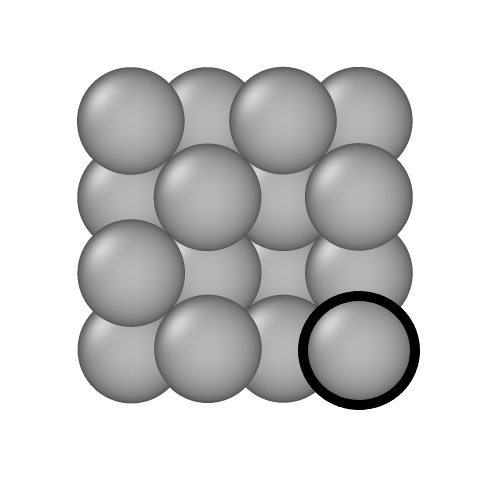
\includegraphics[width=1.5in]{0}}
\subfloat[]{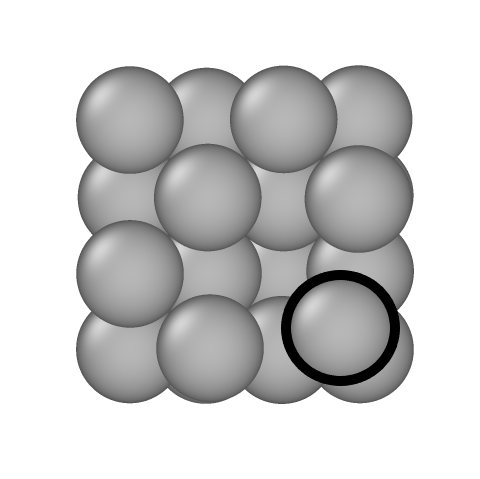
\includegraphics[width=1.5in]{1}}
\subfloat[]{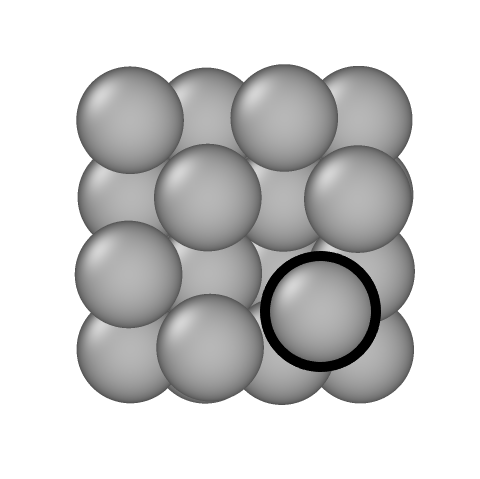
\includegraphics[width=1.5in]{2}}\hfill
\subfloat[]{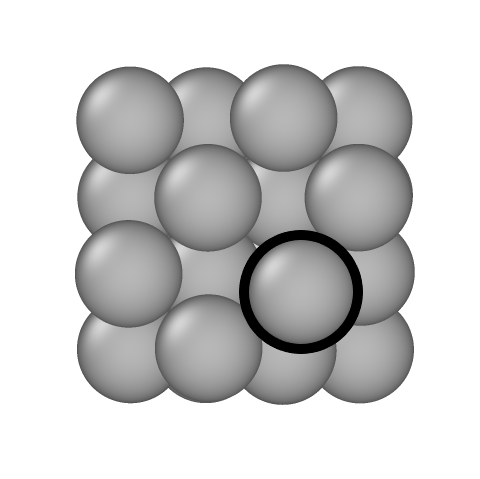
\includegraphics[width=1.5in]{3}}
\subfloat[]{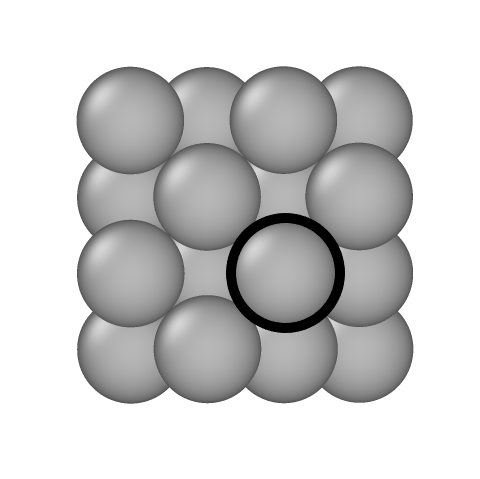
\includegraphics[width=1.5in]{4}}
\caption{Self-diffusion in FCC Aluminum. The migrating atom moves from (a) to (e) via the vacancy mechanism.}
\label{fig:1}
\end{figure}

\section{Background and literature}

\subsection{Self-diffusion in metals}

Self-diffusion in a pure metal is mediated by the migration of point defects, like vacancies and self-interstitials \cite{Shewmon2016}. Self-diffusion in Face Centered Cubic (FCC) metals is controlled by the vacancy mechanism \cite{Mehrer1978} as the vacancy formation energy in FCC metals is much lower than the self-interstitial formation energy. Self-diffusion in Body Centered Cubic (BCC) metals can proceed via both vacancy and interstitial mechanisms, since their vacancy and self-interstitial formation energies are often comparable to each other \cite{Mendelev2007}. Within this thesis, only self-diffusion via the vacancy mechanism will be considered.

\subsubsection{Vacancy concentration}

Vacancies are formed in crystal structures during the solidification process due to atomic vibrations, local rearrangement of atoms, and during plastic deformations \cite{Ehrhart1992}. At any given temperature up to the melting point, the concentration of vacancies $C_v$ in a material is given by,
%
\begin{equation} \label{eq:1}
C_v = \exp\left(\dfrac{-G^v_f}{k_B T}\right) = \exp\left(-\dfrac{H^v_f}{k_B T}\right) \exp\left(\dfrac{S^v_f}{k_B}\right)
\end{equation}
%
where $G^v_f$ is the Gibbs free energy of vacancy formation, $H^v_f$ is the enthalpy of vacancy formation, $S^v_f$ is the vibrational entropy of vacancy formation, $k_B$ is the Boltzmann constant and $T$ is the temperature. 

The vacancy concentration is maximum close to its melting temperature ($\approx10^{-4}$) and decreases drastically with decreasing temperature \cite{Gottstein2004}. Therefore, at any given temperature there will be a finite number of vacancies in a metal at thermodynamic equilibrium.

\subsubsection{Atomic jump process}

At finite temperatures, atoms in a crystal oscillate around their equilibrium positions. For any given atom to \enquote{jump} from its lattice site to a neighboring vacancy site, energy is required. Usually, the oscillations are not violent enough to overcome the barrier and the atom will return to its initial position, since he energy required for a successful jump is typically large with respect to the thermal energy, $k_BT$.  Occasionally, large displacements from the equilibrium position result in a successful jump of the atom to the vacancy site. These activation events are infrequent relative to the frequencies of the lattice vibrations, which are characterized by the Debye frequency. When an atom performs a successful jump it loses its energy and becomes deactivated, and waits on the average for many lattice vibrations before it can jump again. Thus, diffusion of atoms in a crystal occurs in a series of discrete jumps from one lattice site to the next \cite{Mehrer2007}.

The frequency of successful jumps to a vacant nearest neighbor lattice site, or simply the jump frequency $\Gamma$, can be obtained from Eyring's reaction rate theory \cite{Eyring1935} as,
%
\begin{equation} \label{eq:2}
\Gamma = \dfrac{\kappa k_B T}{h} \exp\left(\dfrac{-G^v_m}{k_B T}\right) =\dfrac{k_B T}{h} \exp\left(-\dfrac{H^v_m}{k_B T}\right) \exp\left(\dfrac{S^v_m}{k_B}\right)
\end{equation}
%
where $G^v_m$ is the Gibbs free energy of vacancy migration, $H^v_m$ is the enthalpy of vacancy migration, $S^v_m$, the vibrational entropy of vacancy migration, $h$ is the Planck's constant and $\kappa$ is transmission coefficient, which is the probability that a system reaching the saddle state will proceed to complete the reaction. For self-diffusion, $\kappa=1$ is assumed, such that once an atom gains thermal energy greater than the migration barrier, it always jumps to the vacancy site.

However, a jump can only be successful if the nearest neighbor lattice site is empty, i.e. if it is occupied by a vacancy. If an atom has $z$ nearest neighbors, then the probability that any of the next neighbor sites is vacant is $z C_v$. The self-diffusion coefficient $D$ is given by \cite{Gottstein2004},
%
\begin{equation} \label{eq:3}
D = \dfrac{\lambda^2}{6} \Gamma z C_v 
\end{equation}
%
where $\lambda^2$ is the jump distance.

\begin{figure}[htp] 
\centering
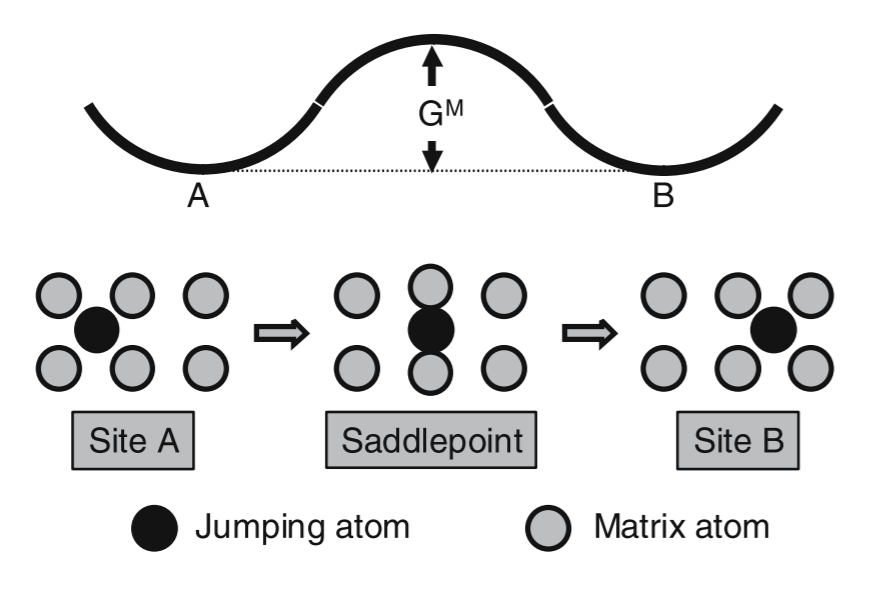
\includegraphics[scale=0.7]{jumping_atom}
\caption{Atomic jump process in a crystalline solid: the black atom moves from an initial configuration (left) to a final configuration (right) pushing through a saddlepoint configuration (middle). Used with permission from \cite{Mehrer2007}.}
\label{fig:2}
\end{figure}

\subsubsection{Correlation factor}

Successive atomic jumps are not truly random. Once an atom jumps to a vacancy site, there is a higher probability that its next jump will be to its previous lattice site than to any of the other neighboring vacancy sites \cite{Leclaire}. The calculated self-diffusion coefficeint $D$ and the actual self-diffusion coefficient $D^*$ are then related by the correlation factor $f$ as,
%
\begin{equation} \label{eq:4}
D^* = fD
\end{equation}
%
The jump correlation factor is 0.78145 for FCC, 0.72149 for BCC \cite{Montet1973}. 

\subsubsection{Random walk}

Another way of obtaining the self-diffusion coefficient in a crystal lattice using simulaiton is by considering diffusion as a random walk problem. The total displacement of an atom is composed of many random individual jumps where it exchanges position with a vacancy at a nearest neighbor site. The mean square displacement $\langle \bm{r}(t)^2 \rangle$ of all the atoms in the crystal and the self-diffusion coefficient are related by a modified version of the Einstein-Smoluchowski relation \cite{VonSmoluchowski1906} as,
%
\begin{equation} \label{eq:5}
D = \dfrac{\langle \bm{r}(t)^2 \rangle}{6\tau} \cdot \dfrac{C_v}{C_v^{cell}}
\end{equation}
%
where $\tau$ is the total time over which diffusion is simulated, and $C_v^{cell}$ is the vacancy concentration of the simulation box. The factor 6 accounts for the translational and vibrational degrees of freedom in 3 dimensions.\\

Eqs. (\ref{eq:3}) and (\ref{eq:5}) show two different approaches to calculating the self-diffusion coefficient. Two common approaches using these equations are the quasi-harmonic method and direct molecular dynamics, respectively. These are discussed presently.

\subsection{The quasi-harmonic method} 

The quasi-harmonic method obtains the self-diffusion coefficient as a solution to Eq. (\ref{eq:3}). The quasi-harmoninc temperature dependent lattice constants are obtained by applying the harmonic approximation at a set of discreet volumes. By performing harmonic approximation at each of these lattice constants, the free energy of vacancy formation used to compute the vacancy concentration is obtained. The phonons from this approximation are then used to compute the attempt frequency using Vineyard's transition state theory \cite{Vineyard1957}, and the migraiton enthalpy is determined using the nudged elastic band method \cite{Henkelman2000}.

\subsubsection{Vineyard's approximation}

\noindent The attempt frequency term $\kappa k_BT/h$, within Eyring's reaction rate theory is based on the assumption that atomic migration is a one-body problem. Though only a single atom performs the jump, it interacts with its surrounding atoms. The treatment of atomic migration as a many-body problem to derive a more complete expression for atomic jump frequency is done in Vineyard's more sophisticated approximation for transition state theory (TST). According to Vineyard's approximation, for a system with N atoms in 3N-dimensional configuration space, the jump frequency $\Gamma$ in Eq. (\ref{eq:2}) is given by,

%
\begin{equation} \label{eq:6}
\Gamma = \dfrac{\displaystyle \prod_{i=1}^{3N-3}\nu_i}{\displaystyle \prod_{i=1}^{3N-4}\nu_i^\prime} \exp\left(\dfrac{-H^v_m}{k_BT}\right)
\end{equation}
%
where $H^v_m$ is the enthalpy of vacancy migration, $\nu_i$ and $\nu_i^\prime$ are the phonon frequencies of the $i^{th}$ atomin the equilibrium state and the transition state respectively. The imaginary frequency of the unstable vibration mode of the transition state due to negative curvature of the energy-diagram for motion in the direction of motion of the vacancy, is excluded from the product in the denominator.

\subsubsection{Quasi-Harmonic Approximation (QHA)} 

\noindent The energetics computed at $T=0$K using an appropriate potential are scaled to finite temperatures using the quasi-harmonic approximation. By making small displacements to the atoms in the equilibrium state, where the force/energy response is well approximated by a harmonic potential, phonons are calculated. This forms the \enquote*{harmonic} part of the QHA. By considering harmonic approximation at the different volumes resulting from these displacements, a volume dependence in the phonon free energy description can be obtained by,
%
\begin{equation} \label{eq:7}
F^{\mathrm{phonon}}(T, V) = k_B T\sum_{i=1}^{3N} \ln \left[2 \sinh \left(\dfrac{h \upsilon_i(V)}{k_B T}\right)\right]
\end{equation}
%
The Gibbs free energy $G$ resulting from this approximation is given by
%
\begin{equation} \label{eq:8}
G(T)=\min_{V}[E^{\mathrm{static}}(V) +  F^{\mathrm{phonon}}(T, V) + PV]
\end{equation}
%
where $E^{\mathrm{static}}$ is the electronic ground state energy at volume $V$ and pressure $P$, $N$ is the number of dynamic atoms in the system, $\upsilon_i$ is the normal phonon frequency for the $i^{th}$ atom, and $h$ is the Planck's constant. 

By increasing the temperature, the volume dependence of the phonon free energy changes and as a result, the equilibrium volume at different temperatures changes. This is considered as thermal expansion under this approximation \cite{Togo2010}. Given a bulk structure and the same structure with a single vacancy, temperature and volume dependent free energies for both structures can be obtained from QHA. The temperature dependent free energy of vacancy formation $G^v_f$ used in Eq. (\ref{eq:1}) is evaluated by the relation,
%
\begin{equation} \label{eq:9}
G^v_f(T) = G_v(T)  - \dfrac{(N - 1)}{N} G_b(T)
\end{equation}
%
where $G_v$ is the Gibbs free energy of the vacancy structure and $G_b$ is the Gibbs free energy of the bulk structure. 

\subsubsection{The Nudged Elastic Band (NEB) method} 

\noindent TST requires the transition state configuration, which is essential to determine the quantities entering Eq. \ref{eq:6}. This transition state can be determined by using the Nudged Elastic Band method \cite{JONSSON1998}. The NEB method is used to find the transition state between any two equilibrium states and determines the Minimum Energy Path (MEP) between these two states. In the case of two equilibrium crystal structures at their respective minimum energies, it gives the \enquote*{saddle point} structure. Several \enquote*{images} are interpolated along the trajectory between these two endpoint structures. The images are assumed to be connected by springs – like an elastic band – to ensure that they do not relax to the minimum energy structures. There are then two forces acting on the atoms within each image – the true force (between atoms within the same image, due to the interatomic potential) and the spring force (between each atom and that same atom's representation in the adjacent images). 

The iterative minimization of these forces, leads to the MEP since the images move to their respective force minima. To ensure that the spring forces do not interfere with the convergence of the images to the MEP and the true force does not affect the distribution of the images along the MEP, a force projection is considered \cite{Henkelman2000}. This force projection $\bm{f}_{\alpha}$ for each image $\alpha$ includes only the parallel component of the spring force $\bm{f}^s|_\parallel$ and the perpendicular component of the true force $-\nabla E(\bm{x}_{\alpha})|_\perp$ to the adjacent images, and is given by,
%
\begin{equation} \label{eq:10}
\bm{f}_{\alpha} = \bm{f}^s|_\parallel -\nabla E(\bm{x}_{\alpha})|_\perp
\end{equation}
%
This results in a “nudge”, which pushes the image towards its force minima \cite{Henkelman2000}. The image with the highest energy is, however, made to climb up along the elastic band to converge rigorously on the highest saddle point. The force projection ${{\bm{f}}_{\alpha}}_{max}$ on this image is,
 %
\begin{equation} \label{eq:11}
{\bm{{f}}_{\alpha}}_{max} = -\nabla E(\bm{x}_{\alpha})|_\perp +\nabla E(\bm{x}_{\alpha})|_\parallel
\end{equation}
%
which is the full force due to the potential, with the component along the elastic band inverted. The highest energy image is not affected by the spring forces at all. The \enquote*{climbing image} moves up the potential energy surface along the elastic band to maximize its energy along the band, and down the potential surface to minimize in all other \cite{Henkelman2000a}. When this image converges, it will be at the exact saddle point.

\begin{figure}[htp]
\centering
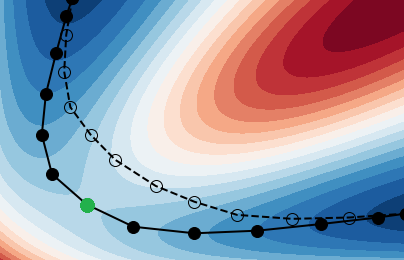
\includegraphics[scale=1.2]{neb}
\caption{An initial band (dotted line) interpolated between the energy minima on a energy landscape converges to the minimum energy path (solid line) using the NEB method. The blue and red areas of the energy landscape represent the low and high energy configurations respectively. The \enquote*{climbing image} is colored green.}
 \label{fig:3}
\end{figure}

Given two structures at equilibrium, one with a vacancy at lattice site $m$ and the other with a vacancy at an adjacent lattice site $m+1$, the NEB method can be used to find the saddle point structure along the trajectory at a given volume. The same method can be repeated for vacancy structures at volumes $V(T)$, to give saddle point structures for each temperature. Since the NEB arranges itself along the MEP, the difference between the total energies of the vacancy structure and its respective saddle point structure at a particular temperature gives the migration enthalpy $H^v_m$ at that temperature, which is used in Eq. (\ref{eq:6}). \\

It is thus possible to compute all the quantities entering Eq. (\ref{eq:3}) and determine temperature dependent self-diffusion coefficients by using QHA and NEB in tandem, which we refer to here as the quasi-harmonic method.

\subsubsection{Drawbacks} 

\noindent Although QHA accounts for thermal expansion of the structure as a whole, it does not account for the local thermal expansion in the lattice regions around the defect, which may be somewhat different from the overall expansion and can become significant as anharmonicity kicks in at increased temperatures. At high temperatures, the amplitudes of the individual atomic vibrations can become so large, that the assumed quadratic expansion of energy at each temperature is no longer adequate. Therefore, QHA can only be considered accurate at relatively low temperatures \cite{Mendelev2009}.

The MEP obtained from the NEB method depends on local characteristics of the potential energy landscape, wherein the path is always parallel to the energy gradient. Non-local features in the direction perpendicular to the path which may arise due to anharmonic vibrations at higher temperatures are not accounted for. As temperature increases from $0K$, the minimum energy path does not necessarily remain the minimum free energy path due to increasing entropic effects \cite{Vanden-Eijnden2009}, corrections for which are not included in the quasi-harmonic method.

\subsection{Molecular dynamics (MD)}

Self-diffusion coefficients from molecular dynamics simulations are obtained directly as a solution to Eq. (\ref{eq:5}): by running an MD simulation as an NPT ensemble, temperature dependent lattice constants can be computed. These lattice constants can then be used to create structures with a single vacancy, and run as an NVT ensemble to compute the mean square displacement of the atoms in the structure at the respective temperature. The free energy of vacancy formation can be computed using thermodynamic integration, a method which will be elaborated in section 3.4.

MD is useful in computing self-diffusion coefficients from fitted classical potentials, as large simulation boxes with many thousands of atoms can be run quickly without much computational cost. Because MD simulates atomic vibrations, anharmonic and non-local entropic effects are captured, which is what makes this method qualitatively better than the quasi-harmonic method at temperatures where anharmonic contributions play a significant role.

\subsubsection{Drawbacks}

\noindent At high temperatures, the jump rates of defects in crystals are within the time scale accessible by running MD. However, as temperature decreases, these jumps rates go beyond this time scale and cannot be simulated without very large computational expense ($\approx$1 jump every 100 ns at 40\% of $T_m$). Hence, MD with classical potentials can be used to compute self diffusion coefficients in metals only at temperatures which are a significant fraction of that metal's melting point \cite{Mendelev2009}. 

Till date, only fully anharmonic vacancy formation energies have been computed for small simulation cells using DFT potentials \cite{Glensk2013}. Even at high temperatures, it is computationally very expensive to calculate self-diffusion coefficients by running MD with DFT potentials for simulation cells greater than 3x3x3 (supercell). Quantum mechanically accurate self-diffusion coefficients beyond very low temperatures are thus difficult to obtain.

\subsection{An alternate approach - The Finite Temperature String (FTS) method}

A alternate method for computing self-diffusion coefficients is the Finite Temperature String (FTS) method \cite{Weinan2005, Vanden-Eijnden2009}. The FTS method is a method for the study of rare events such as conformation changes in molecules, chemical reactions, kinetic phase transitions etc., all of which are activated processes. The mechanisms of such processes can be explained by identifying the path along which this process takes place. Since diffusion is also an activated process, this method can in theory, be used to compute self-diffusion coefficients. For a system with two stable states with several unstable states in between, the Boltzmann-Gibbs distribution gives the probability that a system will be in a certain state as a function of the energy of that state and the temperature of the system. A principle curve \cite{Hastie1989} calculated from such a distribution gives the transition pathway between the two stable states. 

In general, a principal curve is such that its intersection with each of the hyperplanes perpendicular to itself in some appropriate metric coincides with the averaged position of the system in these planes \cite{Hastie1989}. As a result, the principal curves tend to follow low lying channels on the underlying energy or free energy landscapes and, unlike more standard paths such as the minimum energy path or the minimum free energy path, their location depends more globally on the properties of these landscapes. In particular, they permit the smoothing out of the features of the landscape that are below the thermal energy scale and account for non-local contributions related to the width of the channels. It can thereby remain appropriate in situations where the landscape is rough due to thermal fluctuations, anharmonicity and/or non-local entropic effects, as illustrated in Fig. \ref{fig:5}. This was the original formulation of the FTS method \cite{Weinan2005}.

\begin{figure}[htp]
\centering
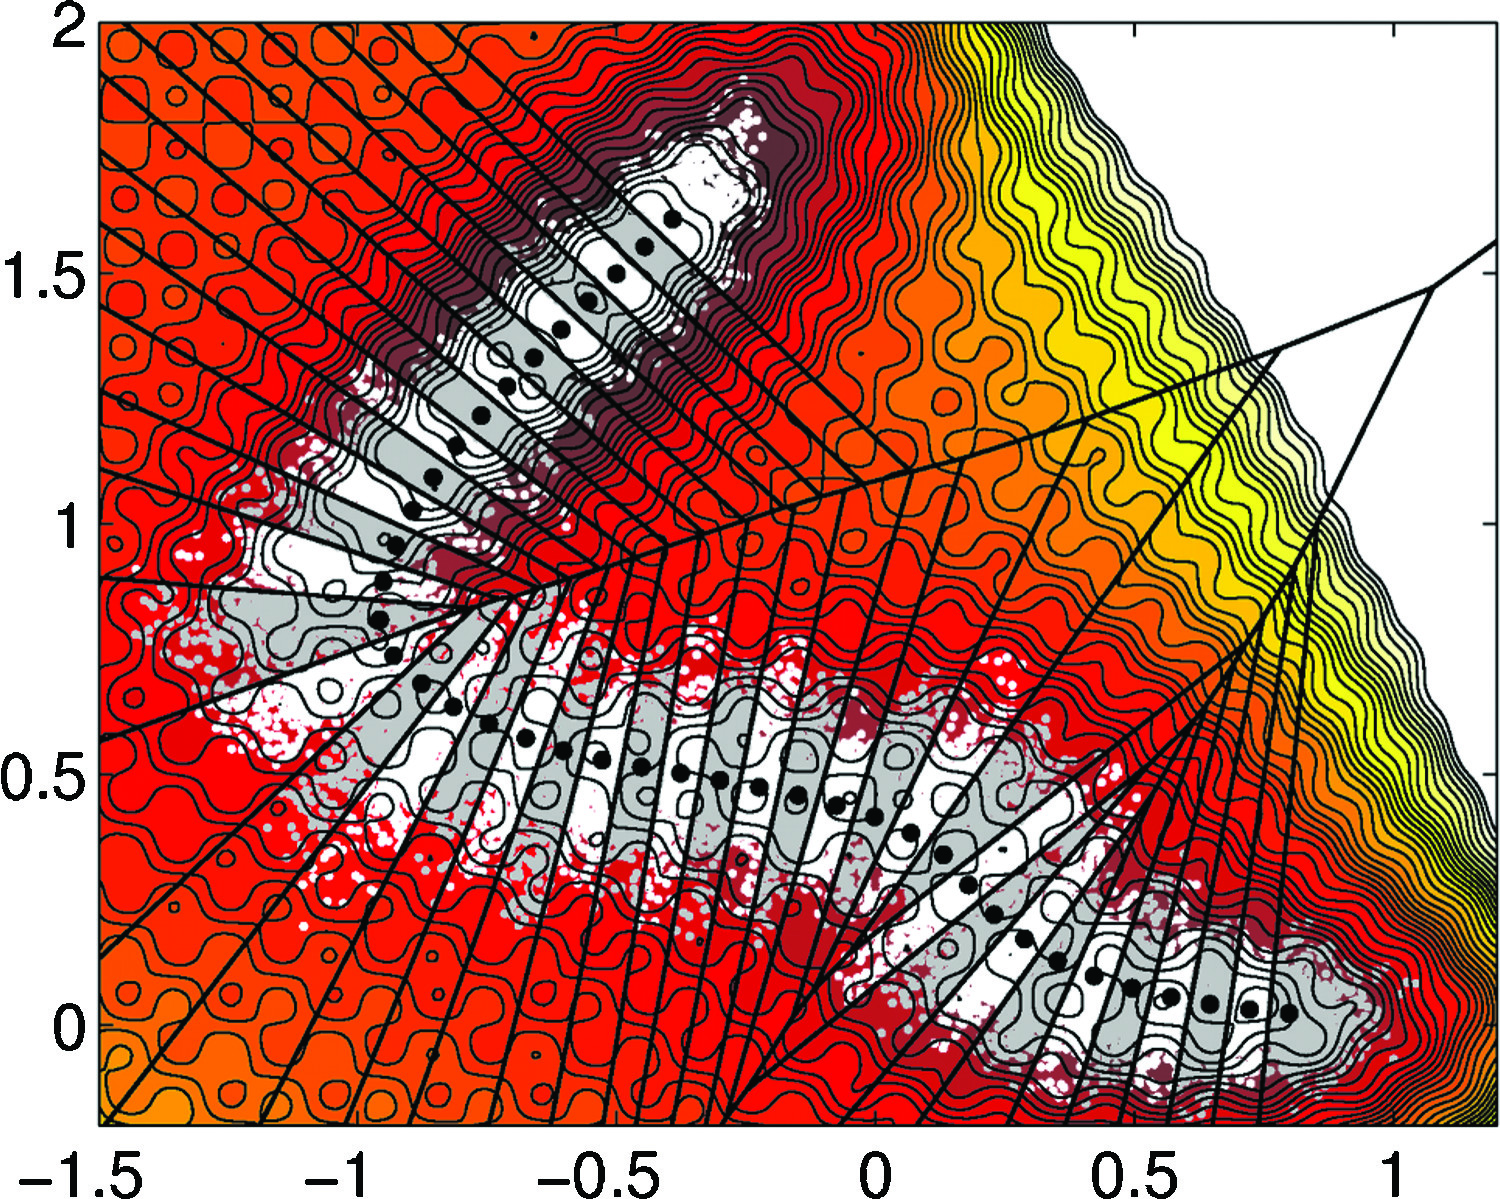
\includegraphics[scale=1.2]{MEP_fts}
\caption{The principal curve (black dots) of the finite temperature string method converges to the reaction tube (white/grey areas) on a rough energy landscape. The sections within black lines are the Voronoi cells within which the system is sampled using MD. Figure used with permission from \cite{Vanden-Eijnden2009}.}
 \label{fig:4}
\end{figure}

An improvement to method, which eliminates the hyperplanes used in the original formulation replaces these planes by Voronoi cells. The principal curve or \enquote*{string} is calculated simply sampling the system using MD constrained within Voronoi cells, whose generating points are the \enquote*{centroids} along the string. Each Voronoi cell comprises of the region in configuration space that is closer to its generating centroid than to any other centroid along the string. The Voronoi cells converge toward the original planes in the limit of infinitely many centroids along the string. When the number of centroids along the string is finite, however, using Voronoi cells rather than planes permits to simplify the FTS algorithm at the cost of a higher computational expense. The distribution of samples within each of the Voronoi cells forms a single \enquote*{reaction tube} within which the transition can be said to occur. The FTS method will, however, fail if this single tube bifurcates, as both the branches will have the same probability of being the transition path. Thus accurate convergence to either one of the branches will not be achieved.

By employing a collision rule at the boundaries of the cells to keep the trajectory inside these cells, while at the same time moving the cells consistently with the sampling output, the centroids can be dragged to the most stable configuration within its respective confines \cite{Vanden-Eijnden2009}. The \enquote*{converged} string is thus along the expected path that the system would take to get from one stable state to another at a given temperature.

Integrating the forces along each centroid configuration up to the saddle point (transition state) gives the \enquote*{virtual work} done by the system to get from the stable state to the saddle point \cite{Swinburne2017}, which is by definition of free energy, the free energy of moving from the stable state to the saddle point. Alternatively, by keeping track of the number of times any given state attempts to change to any another state, and the time between each successive attempt, it is possible to determine the rate at which a system changes from one state to another by the \enquote*{Markovian milestoning} \cite{Vanden-Eijnden2009a} technique.

If applied to two structures at equilibrium, one with a vacancy at lattice site $m$ and the other with a vacancy at an adjacent lattice site $m+1$ at a given temperature, the transition path is obtained from the FTS method. From this path, the free energy of vacancy migration can be computed using the virtual work principle. Independent of the converged string of the FTS method, the jump frequency (or rate of transition) of the migrating atom can be computed directly using the milestoning technique. By obtaining the temperature dependent lattice constant from a regular MD simulation, and the free energy of vacancy formation from thermodynamic integration, fully anharmonic self-diffusion coefficients can be computed using Eq. (\ref{eq:3}).

\begin{figure}[htp]
\centering
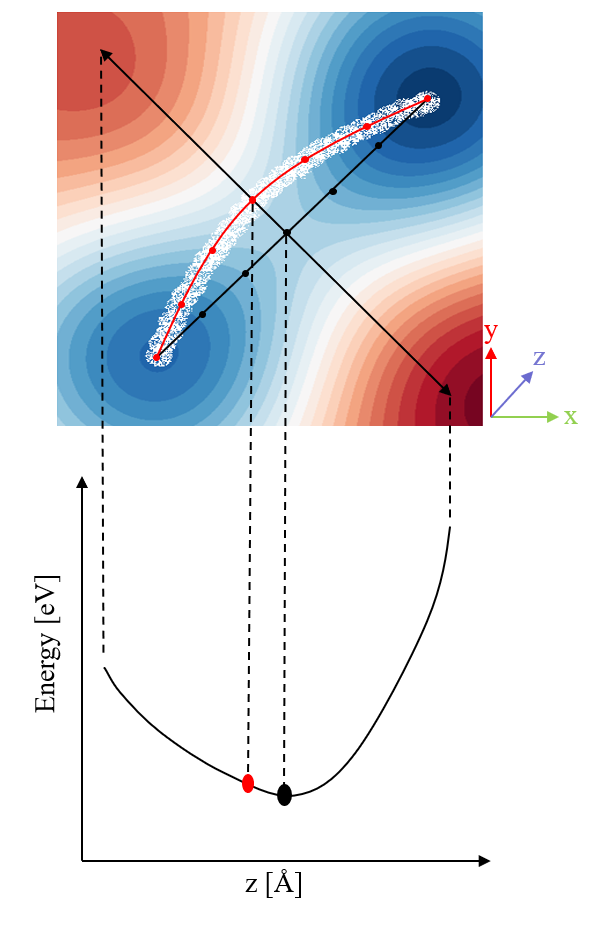
\includegraphics{FTS_anharmonic}
\caption{On an anharmonic energy landscape (along the z-direction), NEB (black line with 7 black points) takes the minimum energy path, ignoring the anharmonicity in the top left corner. FTS (red line with 7 red dots) on the other hand, evolves towards this anharmonicity. The blue and red areas of the energy landscape represent the low and high energy configurations respectively.}
\label{fig:5}
\end{figure}

\newpage

\section{Methods}

Our implementation of the Finite Temperature String (FTS) method comprises of a main module, \enquote*{string evolution}, after which two sub-modules - \enquote*{virtual work} and \enquote*{milestoning} can be used independently of each other to obtain jump frequencies at different temperatures. A separate sub-module for \enquote*{thermodynamic integration} is used to compute the free energy of vacancy formation. This chapter elaborates on the underlying principles of each of these modules in detail.

The mathematical algorithm for the string evolution module was developed by Weinan E., Weiqing Ren and Eric Vanden-Eijnden \cite{Weinan2005} and improved upon by Eric Vanden-Eijnden and Maddalena Venturoli \cite{Vanden-Eijnden2009}. The algorithm for Markovian milestoning was also developed by Eric Vanden-Eijnden and Maddalena Venturoli \cite{Vanden-Eijnden2009a}. Free energies of vacancy formation are computed following the work of de Koning et al. \cite{deKoning}. This thesis implements these methods and combines them to compute fully anharmonic self-diffusion coefficients. The explanations to follow are paraphrased from the above mentioned papers to fit them to this application.

\subsection{String evolution} \label{string_evo}
\label{sec:3.1}

The string evolution module implements the bulk of the FTS method. The objective of this module is to evolve the string while controlling its parameterization until the string converges to the transition path. For two stable states, in this case two equilibrium vacancy structures at their respective energy minima, one with a vacancy at lattice site $m$ and the other with a vacancy at an adjacent lattice site $m+1$, this string is the path along which the vacancy migrates at a given temperature. The flowchart of the string evolution algorithm is shown in Fig. \ref{fig:5}. Each of the nodes is briefly explained with the relevant mathematical notation.

\paragraph*{Initialization:}

During initialization, the initial structure (structure with a vacancy at lattice site $m$), the final strcuture (structure with a vacancy at an adjacent lattice site $m+1$), the semi-empirical interatomic potential (e.g. EAM potential), the number of centroid configurations $(N + 1)$ to be interpolated along the trajectory and the necessary parameters for the subsequent steps (which will be addressed in the steps where they are used) are defined. 

\paragraph*{Interpolation:}

Since the diffusion of a single vacancy is considered, the position of the migrating atom is interpolated between the initial and the final structure, corresponding to the number of initialized centroid configurations. The position vectors of each of these interpolated structures shall be henceforth referred to as \enquote*{centroids}. Throughout this section, boldface characters are used to denote vectors and normal characters to denote their components.

An initial set of $N + 1$ centroids $\bm{\varphi}_{\alpha}^0$ with $\alpha=0,...,N$ is obtained, such that $\mathopen|\bm{\varphi}_{\alpha + 1}^0 - \bm{\varphi}_{\alpha}^0\mathclose| = \mathopen|\bm{\varphi}_{\alpha}^0 - \bm{\varphi}_{\alpha - 1}^0\mathclose|$ for all $\alpha=1,...,(N -1)$. With every centroid $\bm{\varphi}_{\alpha}^0$, an associated \enquote*{image} $\bm{x}_{\alpha}^0$ is set such that $\bm{\varphi}_{\alpha}^0 = \bm{x}_{\alpha}^0$ initially.

For each centroid $\bm{\varphi}_{\alpha}$ along the string, a Voronoi cell $B_{\alpha}$ is defined. $B_{\alpha}$ contains all the coordinates $\bm{x}$ which are closer to its generating centroid $\bm{\varphi}_{\alpha}$ than any other centroid $\bm{\varphi}_{\alpha}^{\prime}$ along the string. For an MD step $n$ at time $t$, this is mathematically represented as,
%
\begin{equation} \label{eq:12}
B_{\alpha}^n = \{\bm{x} \text{ such that } \mathopen|\bm{x} - \bm{\varphi}_{\alpha}^n\mathclose| < \mathopen|\bm{x} - \bm{\varphi}_{\alpha^\prime}^n\mathclose| \text{ for all } \alpha^{\prime} \ne \alpha \}
\end{equation}
%

\begin{figure}
\begin{center}
\begin{tikzpicture}[node distance=2cm, auto]

\node (start)  	[startstop]  								{\small Start};
\node (pro1) 	[process, right of=start, xshift=1.7cm]  		{\small Initialization};
\node (pro2)		[process, right of=pro1, xshift=1.7cm]		{\small Interpolation};
\node (pro3)		[process, right of=pro2, xshift=1.7cm]		{\small Initialize velocities};
\node (dec1)		[decision, below of=pro3, yshift=-0.5cm]	{\small Convergence};
\node (pro4)		[process, left of=dec1, xshift=-2.75cm]		{\small Thermostat};
\node (pro5)		[process, below of=pro4, yshift=0.5cm]		{\small Reflect};
\node (dec2)		[decision, left of=pro4, xshift=-2.25cm]		{\small Thermalization};
\node (pro6)		[process, below of=dec2, yshift=-3cm]		{\small Running average};
\node (dec3)		[decision, right of=pro6, xshift=2.25cm]	{\small Sampling};
\node (pro7)		[process, below of=dec3, yshift=-0.75cm]	{\small Mix};
\node (pro8)		[process, below of=pro7]					{\small Smooth};
\node (pro9)		[process, below of=pro8]					{\small Reparameterize};
\node (pro10)	[process, below of=pro9]					{\small Centroid forces};
\node (pro11)	[process, below of=pro10]					{\small Recenter};
\node (stop)  	[startstop, below of=dec1, yshift=-3.5cm]  	{\small Stop};

\draw [arrow] (start) -- (pro1);
\draw [arrow] (pro1) -- (pro2);
\draw [arrow] (pro2) -- (pro3);
\draw [arrow] (pro3) -- (dec1);
\draw [arrow] (dec1) -- node [midway, below] {False} (pro4);
\draw [arrow] (pro4) -- (pro5);
\draw [arrow] (pro5.west) -| ++ (-0.5,1.5) -- (dec2.east);
\draw [arrow] (dec2.west) -| ++ (-0.5,-5) node[midway, left] {True} -- (pro6.west);
\draw [arrow] (dec2.south) |- ++ (9.5, -1) node[midway, left] {False} -- (dec1.south);
\draw [arrow] (dec3) -- node[midway, right] {True} (pro7);
\draw [arrow] (dec3.north) |- ++ (4.75, 0.5) node[midway, left] {False} -- (dec1.south);
\draw [arrow] (pro6) -- (dec3.west);
\draw [arrow] (pro7) -- (pro8);
\draw [arrow] (pro8) -- (pro9);
\draw [arrow] (pro9) -- (pro10);
\draw [arrow] (pro10) -- (pro11);
\draw [arrow] (pro11.east) -| ++ (0.5, 12) -- ++ (2.72, 0) -- (dec1.south);
\draw [arrow] (dec1.east) -| ++ (0.5, -5.5) node [midway, right] {True} --  (stop.east);

\end{tikzpicture}
\end{center}
\caption{The string evolution flowchart}
\label{fig:6}
\end{figure}

\paragraph*{Initialize velocities:}

Each image is then assigned an initial velocity $\bm{v}_{\alpha}^0$ where $\alpha=0,...,N$ from the Maxwell distribution corresponding to a desired temperature $T$. A center of mass correction is applied to each of these velocities, such that there is no translational drift \cite{Bender2000}. \\

\noindent A set of initial static computations are performed with each image as an input, to obtain the initial forces $\bm{f}_{\alpha}^0$ where $\alpha=0,...,N$, for each image. 

\paragraph*{Convergence:}

A convergence check is performed. The convergence criterion for string evolution is the following,
%
\begin{equation} \label{eq:13}
\mathopen|\{\bm{\varphi}_{\alpha}^{n+1} - \bm{\varphi}_{\alpha}^{n}\}\mathclose|_{\alpha=0,...,N} \leq c
\end{equation}
%
where $c$ in the tolerance limit, and $n+1$ is the MD step corresponding to time $t+\Delta t$. If this criterion is not satisfied, the next node is executed. If it is satisfied, the computation is stopped. Another exit criterion can be the number of maximum steps over which to evolve the string, which is helpful for testing and debugging.

\paragraph*{Thermostat:}

A thermostat is used to give each of the atoms of an image a \enquote*{kick} in a random direction. This kick corresponds to the Maxwell distribution at the temperature $T$ specified earlier. In this thesis, a Langevin thermostat \cite{Davidchack2009} is used. In addition to giving a random kick, this thermostat also introduces a \enquote*{drag} to simulate the viscous aspect of a fluid. A velocity verlet algorithm \cite{Swope1982} is used for simulating Langevin dynamics. The thermostatting algorithm has three steps:

\begin{description}
\item[Step 1.] The half-step velocities $\bm{v}_{\alpha}^{**}$ and the new positions $\bm{x}_{\alpha}^*$ for each image are calculated using,
%
\begin{equation} \label{eq:14}
\bm{v}_{\alpha}^{**}\left(t + \dfrac{1}{2}\Delta t\right) = \bm{v} _{\alpha}^n(t) + \dfrac{1}{2}\bm{a}_{\alpha}^n(t)\Delta t
\end{equation}
%
%
\begin{equation} \label{eq:15}
\bm{x}_{\alpha}^*(t + \Delta t) = \bm{x}_{\alpha}^n(t) + \bm{v}_{\alpha}^{**}\left(t + \dfrac{1}{2}\Delta t\right)\Delta t
\end{equation}
%

where $\Delta t$ is the timestep of the thermostat, $\bm{a}_{\alpha}^n$ is the acceleration which is calculated from the forces $\bm{f}_{\alpha}^n$ and the masses of the atomic species $M$.
\end{description}

\begin{description}
\item[Step 2.] Another static computation is performed at the new positions $\bm{x}_{\alpha}^*(t + \Delta t)$ of each image. To the resulting forces $\nabla U(\bm{x}_{\alpha}^*)$ obtained, a kick is added in a random direction and a drag is introduced according to Langevin equation \cite{Schlick2010} giving new forces,
%
\begin{equation} \label{eq:16}
\bm{f}_{\alpha}^*(t + \Delta t) = \nabla U(\bm{x}_{\alpha}^*) - \gamma \bm{v}_{\alpha}^{**}\left(t + \dfrac{1}{2}\Delta t\right)+ \sqrt{2\gamma k_BT}\bm{R}(t)
\end{equation}
%
where $\gamma$ is the damping factor of the thermostat corresponding to the drag, $k_B$ is the Boltzmann constant and $\bm{R}(t)$ is a delta-correlated stationary Gaussian process having a mean of 0 and variance of 1.
\end{description}

\begin{description}
\item[Step 3.] The full-step velocities $\bm{v}_{\alpha}^*$ for each image are then calculated as,
%
\begin{equation} \label{eq:17}
\bm{v}_{\alpha}^*(t + \Delta t) = \bm{v}_{\alpha}^{**}\left(t + \dfrac{1}{2}\Delta t\right) + \dfrac{1}{2}\bm{a}_{\alpha}^*(t)\Delta t
\end{equation}
%
\indent where $\bm{a}_{\alpha}^*$ is the acceleration calculated from $\bm{f}_{\alpha}^*$.
\end{description}

\paragraph*{Reflect:}

$\bm{x}_{\alpha}^*$, $\bm{v}_{\alpha}^*$ and $\bm{f}_{\alpha}^*$ are temporary positions, velocities and forces. The update from step $n$ to step ${n+1}$ depends on the boundary condition, at which the collision rule is applied. The boundary condition for an image is given by,
%
\begin{numcases}{\bm{x}_{\alpha}^{n+1}=} \label{eq:18}
\bm{x}_{\alpha}^*, & \text{if $\bm{x}_{\alpha}^* \in B_{\alpha}^n$} \\
\bm{x}_{\alpha}^n, & \text{otherwise}
\end{numcases}
%
where $B_{\alpha}^n$ is the Voronoi cell as defined in Eq. (\ref{eq:12}). This is essentially a distance check, to check if each image with new positions $\bm{x}_{\alpha}^*$ is closest to its generating centroid $\bm{\varphi}_{\alpha}^n$. The same condition is also extended to the velocities $\bm{v}_{\alpha}^{*}$ and the forces $\bm{f}_{\alpha}^{*}$ as,
%
\begin{numcases}{\bm{v}_{\alpha}^{n+1}=} \label{eq:20}
\bm{v}_{\alpha}^*, & \text{if $\bm{x}_{\alpha}^* \in B_{\alpha}^n$} \\
-\bm{v}_{\alpha}^n, & \text{otherwise}
\end{numcases}
%
%
\begin{numcases}{\bm{f}_{\alpha}^{n+1}=} \label{eq:22}
\bm{f}_{\alpha}^*, & \text{if $\bm{x}_{\alpha}^* \in B_{\alpha}^n$} \\
\bm{f}_{\alpha}^n, & \text{otherwise}
\end{numcases}
%
the difference being that the velocity is reversed. Thus a \enquote*{reflection} off a boundary of the Voronoi cell is simulated.\\

\noindent At high temperatures, any of the nearest neighbor atoms to the vacancy site can move to this site. This is undesirable, as it would modify the configuration of the centroid to one which is not along the trajectory of the migrating atom. For this reason, the atoms which make up each image are further confined, such that no atom moves to the vacancy lattice site. A per atom reflection is employed for this purpose, by specifying a reflection cutoff which is half of the nearest neighbor distance. If the distance between an atom in an image and the same atom in its corresponding centroid is greater than this cutoff, its position, velocity and force are set to its previous position, velocity and force, with the velocity reversed.

\paragraph*{Thermalization:}

A thermalization check is performed to ensure that the simulation has run long enough for system to equilibrate to the temperature that the thermostat simulates. If the number of the present step $n$ is greater than the number of thermalization steps $n_T$ the system is thermalized and the next node is executed. Otherwise, the convergence check is performed again.

\paragraph*{Running average:}

The evolution of the string in the direction of the mean positions of each Voronoi cell is done in two parts: by calculating the running average of the positions of each image, and then mixing a fraction of this running average to the positions of the generating centroid. ~\\

\noindent A running average $\bm{\bar{x}}_{\alpha}^n$ of each $\bm{x}_{\alpha}^n$ is calculated as,
%
\begin{equation} \label{eq:24}
\bm{\bar{x}}_{\alpha}^n =  \dfrac{1}{n - n_T} \sum_{n^{\prime} = n_T}^{n} \bm{x}_{\alpha}^{n^{\prime}}
\end{equation}
%
where $n_T$ is the number of thermalization steps.

\paragraph*{Sampling:}

In order to ensure that enough configuration samples within each Voronoi cell have been included into the running average, a sampling check is performed. This is a modification to the improved FTS algorithm \cite{Vanden-Eijnden2009} made in this thesis. The reason for doing this is that with increasing temperature, the configurational space within a Voronoi cell available to an image to explore grows. The number of samples that then need to be averaged to get an accurate running average configuration within that cell also increases. If the number of the present step is an integer multiple of the number of sample steps, the next node is executed. Otherwise, the subroutine for updating the string centroids is passed over and convergence check is performed again.

\paragraph*{Mix:}

Each centroid along the string is then updated towards the running average $\bm{\bar{x}}_{\alpha}^n$ by mixing the two according to the relation,
%
\begin{equation} \label{eq:25}
\bm{\varphi}_{\alpha}^* = \bm{\varphi}_{\alpha}^n - \Delta \tau (\bm{\varphi}_{\alpha}^n - \bm{\bar{x}}_{\alpha}^n)
\end{equation}
%
where $\Delta \tau$ is the mixing fraction and $0 \leq \Delta \tau \leq 1$, such that $\bm{\varphi}_{\alpha}^*$ is a weighted average between $\bm{\varphi}_{\alpha}^n$ and $\bm{\bar{x}}_{\alpha}^n$, where the relative weight of both terms is controlled by $\Delta \tau$.

\paragraph*{Smooth:}

To keep the updated string relatively smooth despite possible statistical fluctuations in $\bm{\bar{x}}_{\alpha}^n$, the updated centroids $\bm{\varphi}_{\alpha}^*$ are smoothened. A tridiagonal matrix $M_T$, corresponding to the following equation is constructed,
%
\begin{equation} \label{eq:26}
\bm{\lambda}_{\alpha}^* = \kappa (N+1) \Delta \tau (\bm{\varphi}_{\alpha-1}^* -2 \bm{\varphi}_{\alpha}^*+ \bm{\varphi}_{\alpha+1}^* )
\end{equation}
%
where $\kappa$ is the nominal smoothing and $0 \leq \kappa \leq 1$, $\bm{\lambda}_{0}^* = \bm{\lambda}_{N_i}^* = 0$ and $\alpha=1,...,(N -1)$. Here, $\bm{\lambda}_{\alpha}^*$ form the rows of $M_T$.

$M_T$ is a matrix with dimensions $(N \times N)_{ij}$ where $N$ is the number of centroids along the string. $i$ corresponds to an individual centroid, while $j$ is every other centroid along the string, including itself (for $i=j$). $M_T$ represents the influence of each centroid over every other centroid along the string, and not just its left and right neighbors. It is used in order to smoothen each centroid with respect to every other centroid along the string according to $\kappa$, which controls the aggressiveness of the smoothing. Thus, smoothing is done \enquote*{globally}. The smoothed centroids $\bm{\varphi}_{\alpha}^s$ are obtained using the equation,
%
\begin{equation} \label{eq:27}
\bm{\varphi}_{\alpha}^s = \bm{\varphi}_{\alpha}^* (1 - M_T)^{-1}
\end{equation}
% 
Since matrix inversion is computationally expensive, $M_T$ is calculated only once at the beginning of the run, and is then reused for the rest of the simulation, so long as the number of images $N$ and the smoothing strength $\kappa$ are kept constant.

\paragraph*{Reparameterize:}

During string update and smoothing, the centroids along the string are no longer equidistant from each other. In order to enforce equal arc-length parameterization, a piecewise linear curve is interpolated through $\{\bm{\varphi}_{\alpha}^s\}_{\alpha=0,...,N_i}$. If $L(\alpha)$ gives the length up to $\bm{\varphi}_{\alpha}^s$ of the piecewise linear curve, then $L(0) = 0$, and for $\alpha=0,...,N_i$,
%
\begin{equation} \label{eq:28}
L(\alpha) = \sum_{\alpha^{\prime} = 1}^{\alpha} \mathopen|\bm{\varphi}_{\alpha^{\prime}}^{s} - \bm{\varphi}_{\alpha^{\prime}-1}^{s}\mathclose|
\end{equation}
such that $L(N)$ is the total length of the piecewise linear curve, and $l(\alpha) = L(N){\alpha}/N_i$ for $\alpha=0,...,N$ is the distance along this curve from the image $\bm{\varphi}_0^s$ up to the point at which the new $\alpha^{\text{th}}$ image $\bm{\varphi}_{\alpha}^{n+1}$ needs to be set, in order to make the images equidistant along the curve. Setting $\bm{\varphi}_{0}^{n+1} = \bm{\varphi}_{0}^s$ and $\bm{\varphi}_{N}^{n+1} = \bm{\varphi}_{N}^s$, the \enquote*{reparameterized} centroids are given by,
%
\begin{equation} \label{eq:29}
\bm{\varphi}_{\alpha}^{n+1} = \bm{\varphi}_{a(\alpha)-1}^s + (l(\alpha) - L(a(\alpha) -1)) \dfrac{\bm{\varphi}_{a(\alpha)}^s - \bm{\varphi}_{a(\alpha)-1}^s}{\mathopen|\bm{\varphi}_{a(\alpha)-}^s - \bm{\varphi}_{a(\alpha)-1}^s\mathclose|}
\end{equation}
% 
where $a(\alpha)=1,...,N$ is such that $L(a(\alpha) - 1) < l(\alpha) \leq L(a(\alpha))$, and the condition $\mathopen|\bm{\varphi}_{\alpha + 1}^{n+1} - \bm{\varphi}_{\alpha}^{n+1}\mathclose| = \mathopen|\bm{\varphi}_{\alpha}^{n+1} - \bm{\varphi}_{\alpha - 1}^{n+1}\mathclose|$ for all $\alpha=1,...,(N -1)$ is satisfied. \\

\noindent $\bm{\varphi}_{\alpha}^{n+1}$ are now the centroids along the evolved string after a single MD step. From these centroids, new Voronoi cells $B_{\alpha}^{n+1}$ are generated, within which the sampling of running average will continued in the subsequent MD step.

\paragraph*{Centroid forces:}

The forces on each centroid $\bm{f}({\bm{\varphi}_{\alpha}^{n+1}})$, are computed.

\paragraph*{Recenter:}

In order to make sure that the new images $\bm{x}_{\alpha}^{n+1}$ are not outside their new Voronoi cells $B_{\alpha}^{n+1}$, the boundary condition is once again applied such that,
%
\begin{numcases}{\bm{x}_{\alpha}^{n+1}=} \label{eq:30}
\bm{x}_{\alpha}^{n+1}, & \text{if $\bm{x}_{\alpha}^{n+1} \in B_{\alpha}^{n+1}$} \\
\bm{\varphi}_{\alpha}^{n+1}, & \text{otherwise}
\end{numcases}
%
%
\begin{numcases}{\bm{f}_{\alpha}^{n+1}=} \label{eq:32}
\bm{f}_{\alpha}^{n+1}, & \text{if $\bm{x}_{\alpha}^{n+1} \in B_{\alpha}^{n+1}$} \\
\bm{f}({\bm{\varphi}_{\alpha}^{n+1}}) & \text{otherwise}
\end{numcases}
%
\\
Following this node, the convergence check performed.
\\

\noindent If the convergence criterion is satisfied, it can be said that the string has converged to the minimum free energy path along which the atom migrates at the temperature $T$. The centroid configurations along the converged string can be used to compute the free energy of vacancy migration from the virtual work principle, or to compute the jump frequency directly form the Markovian milestoning method.

\subsection{Virtual work principle}

In the context of atomic migration, work is done in moving an atom from one lattice point to an adjacent lattice point with a vacancy. Since work is a path function, it depends not only on the initial and final position of the atom, but also on the path taken by it. Each centroid along the converged string obtained from the string evolution module, is a configuration of the structure around the migrating atom as it migrates. From these centroids it is then possible to compute the \enquote*{virtual work} $W$, in moving the atom from its equilibrium position to the saddle point, and is given by,
%
\begin{equation} \label{eq:34}
W(\bm{\varphi}_{\alpha=0, ..., \mathrm{saddle}}) = - \int_{\bm{\varphi}_{0}}^{\bm{\varphi}_{\mathrm{saddle}}} \bm{f}(\bm{\varphi}_{\alpha}) \cdot d\bm{\varphi}_{\alpha}
\end{equation}
% 
where $\bm{f}(\bm{\varphi}_{\alpha})$ are the forces computed at the converged centroids $\bm{\varphi}_{\alpha}$.

The movement of this atom can be conversely seen as the movement of the associated vacancy. Therefore, the virtual work $W(T)$ done in moving the vacancy from its equilibrium position to its saddle point at a given temperature $T$, by definition of free energy, is the free energy of vacancy migration, $F_{m}^{v}(T)$ at that temperature $T$,
%
\begin{equation} \label{eq:35}
W(T) = F_{m}^{v}(T)
\end{equation}
% 

\noindent The free energy computed from the virtual work method is the Helmholtz free energy, and not the Gibbs free energy. The computation of Gibbs free energy of vacancy migration is computationally taxing, and hence a simplifying assumption is made here, that the Gibbs free energy is very close to the computed Helmholtz free energy.

\subsection{Markovian Milestoning} \label{mile}

Another method to compute the jump frequency in Eq. \ref{eq:3} directly without having to compute the free energy of vacancy migration, is the Markovian milestoning method \cite{Vanden-Eijnden2009a}. Markovian milestoning is a computational procedure which can provide kinetic information of a dynamic system by running constrained molecular dynamics within Voronoi cells. The probability of the system to remain in any given cell can be computed from the rate of entry and exit for each cell. Each edge of a cell is considered a \enquote*{milestone}, which is effectively a boundary in configuration space that separates the configurations in one cell from those in another. When the system changes its configuration from the space represented by one cell to another, the milestone between those two cells is \enquote*{crossed}. The number of times each milestone is crossed by a system after having crossed another milestone is recorded. After crossing this milestone, the time taken by the system to cross the next milestone is also recorded. From this information, statistical methods can be used to access time scales which are typically inaccessible by brute-force molecular dynamics to compute properties such as mean first passage times and the transition rates between the milestones. 

Markovian Milestoning is a technique which does not necessarily require that the centroids of the Voronoi cells are along the transition path. Given a sufficiently long run time, the transition rates computed by this technique will eventually converge to the ones predicted by the FTS method with virtual work. However, using milestoning in conjunction with the FTS method has its advantages: the string method produces cells whose edges are approximations of the isocomittor surfaces, and these surfaces can be considered as \enquote*{optimal milestones} in the sense that transitions between them are statistically independent. This means, in particular, that transition rates between any two cells can be computed exactly by milestoning.

The milestoning sub-module calculates the jump frequency of an atom at a given temperature using an algorithm whose flowchart is shown in Fig. \ref{fig:7}. Nodes which repeat from section \ref{sec:3.1} (string evolution) function the same way as earlier, and will not be explained again. \\

\noindent The sub-module is initialized similar to the string evolution module. Additionally, a new set of $N + 1$ centroids are defined, and are set to the centroids along the converged string. Care must be taken to ensure that the number of centroids for both modules are the same. Since the milestoning technique does not require the centroids to be along the actual transition path, the images from NEB can also be considered as valid centroids. In this work, milestoning with NEB is performed.

An associated image for each centroid is also defined (\textbf{Initialization}). These images are assigned initial velocities (\textbf{Initialize velocities}) and checked for convergence.

\paragraph*{Convergence:}

The convergence criterion for this module is simple a step check: if the number of the present step is greater than or equal to the number of maximum steps specified, the computation is stopped. Since markovian milestoning is a statistical technique, it is essential to have a sufficiently high number of maximum steps in order to obtain results with low error bars. \\

\noindent The nodes \textbf{Thermostat}, \textbf{Reflect} and \textbf{Thermalization} are then executed. If the number of the present step $n$ is greater than the number of thermalization steps $n_T$ the system is thermalized and the next node is executed. Otherwise, the convergence check is performed again.

\paragraph*{Milestone:}

The Voronoi cells generated from the centroids impinge on each other, and share boundaries with other cells forming cell \enquote*{edges}. The total number of edges shared by any cell $B_{\alpha}$ with all the other cells $B_{\alpha^{\prime}}$ is given by,
%
\begin{equation} \label{eq:34}
N_e = \dfrac{(N +1)(N)}{2}
\end{equation}
%
where $N + 1$ is the number of generating points which is this case, are the centroids. These edges form the \enquote*{milestones} within the milestoning technique.\\

\begin{figure}[htp]
\centering
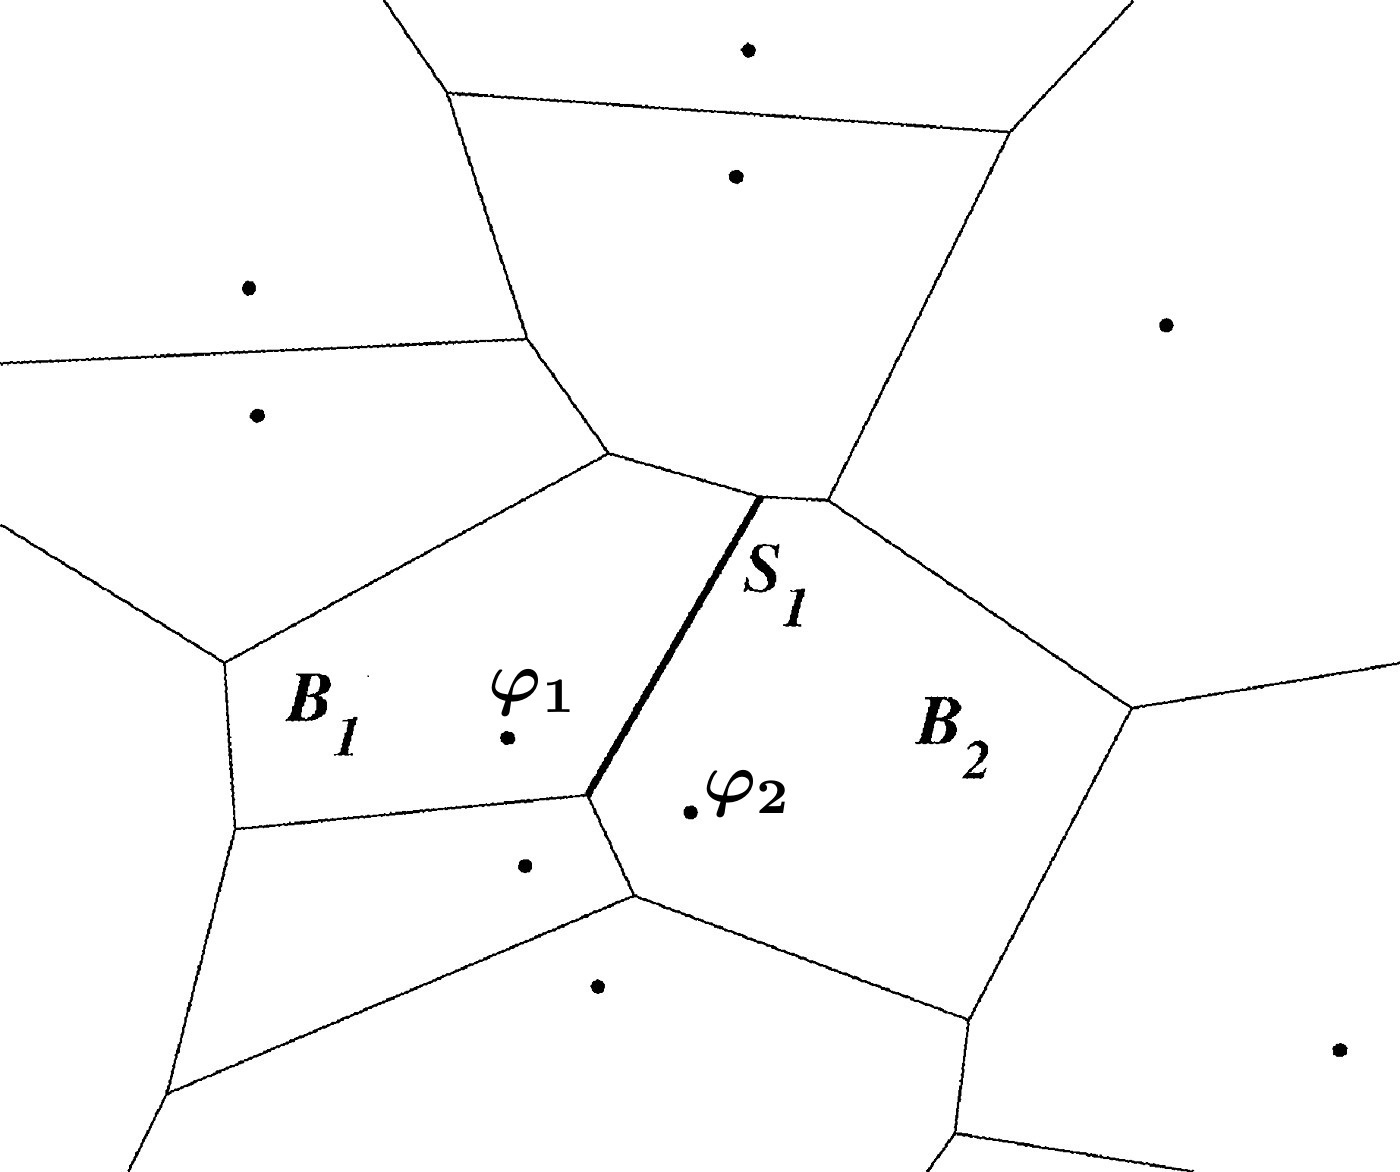
\includegraphics[scale=1.2]{voronoi}
\caption{Voronoi cells ($B_1, B_2$) generated from the centroids ($\bm{\varphi_1}, \bm{\varphi_2}$) respectively, impinge on each other, forming the edge $S_1$. Figure used with permission from \cite{Vanden-Eijnden2009a}.}
 \label{fig:7}
\end{figure}

The number of times $\bm{x}_{\alpha}$, which is restricted to cell $B_{\alpha}$, collides with one of the edges of the cell after having last hit another edge of the cell is recorded by $N_{ij}^{\alpha}$, where $i$ is the edge index of cell $B_{\alpha}$ and $j$ is the edge index of the cell $B_{\alpha^{\prime}}$, with which $B_{\alpha}$ shares this edge. Next, the index of the last edge contacted $i_{\alpha}$ is recorded. $i_{\alpha}$ can only assume values of indices of the edges of $B_{\alpha}$. The total time $\bm{x}_{\alpha}$ spends at $i_{\alpha}$, which is the time elapsed between a collision with one edge and a collision with another edge is recorded, and is denoted by $R_i^{\alpha}$.

Knowing that the total flux in and out of each cell in the system must be zero at statistical steady state, the number of times $\bm{x}_{\alpha}$ tries to jump from cell $B_{\alpha}$ to another cell $B_{\alpha^{\prime}}$ is also recorded as $N_{\alpha, \alpha^{\prime}}$.  \\

\begin{figure}
\begin{center}
\begin{tikzpicture}[node distance=2cm, auto]

\node (start)  	[startstop]  								{\small Start};
\node (pro1) 	[process, right of=start, xshift=1.7cm]  		{\small Initialization};
\node (pro2)		[process, right of=pro1, xshift=1.7cm]		{\small Initialize velocities};
\node (dec1)		[decision, below of=pro2, yshift=-0.5cm]	{\small Convergence};
\node (pro3)		[process, left of=dec1, xshift=-2.5cm]		{\small Thermostat};
\node (pro4)		[process, below of=pro3, yshift=0.5cm]		{\small Reflect};
\node (dec2)		[decision, below of=pro4, yshift=-0.5cm]	{\small Thermalization};
\node (pro5)		[process, below of=dec2, yshift=-2cm]		{\small Milestone};
\node (pro6)		[process, below of=dec1, xshift=3cm]		{\small Post processing};
\node (stop)  	[startstop, below of=pro6, yshift=0.5cm]  	{\small Stop};

\draw [arrow] (start) -- (pro1);
\draw [arrow] (pro1) -- (pro2);
\draw [arrow] (pro2) -- (dec1);
\draw [arrow] (dec1) -- node [midway, below] {False} (pro3);
\draw [arrow] (pro3) -- (pro4);
\draw [arrow] (pro4) -- (dec2);
\draw [arrow] (dec2.west) -| ++ (-0.5,-4) node[midway, left] {True} -- (pro5.west);
\draw [arrow] (dec2.south) |- ++ (4.5, -0.5) node[midway, left] {False} -- (dec1.south);
\draw [arrow] (pro5.east) -| ++ (2.97, 5) -- (dec1.south);
\draw [arrow] (dec1.east) -| ++ (1.46, -1.5) node [midway, right] {True} --  (pro6);
\draw [arrow] (pro6) -- (stop);

\end{tikzpicture}
\end{center}
\caption{The string evolution flowchart}
\label{fig:8}
\end{figure}

\noindent If the computation has run for the number of maximum steps specified, post processing is carried out. Otherwise, the \textbf{Convergence} node is executed once more.

\paragraph*{Post-processing:}

From $N_{\alpha, \alpha^{\prime}}$, the rate of escape $k$ from cell $B_{\alpha}$ to another cell $B_{\alpha^{\prime}}$ can be calculated as,
%
\begin{equation} \label{eq:35}
k_{\alpha, \alpha^{\prime}} = \dfrac{N_{\alpha, \alpha^{\prime}}}{T_{\alpha}}
\end{equation}
%
where $T_{\alpha}$ is the total simulation time in cell $B_{\alpha}$. These rates can then be used to estimate the equilibrium probability $\pi_{\alpha}$ to find a system in the cell $B_{\alpha}$, from the unique solution of,
%
\begin{equation} \label{eq:36}
\sum_{\substack{\alpha^{\prime} = 0 \\ \alpha^{\prime} \neq \alpha}}^{N_i + 1} \pi_{\alpha^{\prime}} k_{\alpha^{\prime}, \alpha} = \sum_{\substack{\alpha^{\prime} = 0 \\ \alpha^{\prime} \neq \alpha}}^{N_i + 1} \pi_{\alpha} k_{\alpha, \alpha^{\prime}} \text{   ,   } \sum_{\alpha = 0}^{N_i + 1} \pi_{\alpha} = 1
\end{equation}
%
which expresses that at statistical steady state, the probability to find the system in cell $B_{\alpha}$ and see it escape to another cell is the same as the probability to find it in another cell and see it enter $B_{\alpha}$.

The total number of collisions from edge $i$ to $j$, $N_{ij}$ and the total time spent at each edge $R_i$ are computed as,
%
\begin{equation} \label{eq:37}
N_{ij} = \sum_{\alpha = 0}^{N_i +1} \pi_{\alpha} \dfrac{N_{ij}^{\alpha}}{T_{\alpha}}
\end{equation}
\begin{equation} \label{eq:38}
R_{i} = \sum_{\alpha = 0}^{N_i +1} \pi_{\alpha} \dfrac{R_{i}^{\alpha}}{T_{\alpha}}
\end{equation}
%

The maximum likelihood estimators \cite{Myung2003} for $N_{ij}$ and $R_i$ are,
%
\begin{equation} \label{eq:39}
p_{ij} =\dfrac{N_{ij}}{\sum_{j}^{N_e} N_{ij}}
\end{equation}
\begin{equation} \label{eq:40}
\tau_{i} =\dfrac{R_{i}}{\sum_{j}^{N_e} N_{ij}}
\end{equation}
%
where $N_{ii} = 0$ by construction. The $N_e \times N_e$ matrix formed by $p_{ij}$ is $P$, and $\tau$ is the $N_e$ long row matrix of $\tau_i$.

If the milestones are labeled such that $S_{N_e}$ is the largest milestone, then the mean first passage time from milestone $S_i$ to $S_N$ can be computed as the solution of,
%
\begin{equation} \label{eq:41}
(\text{Id} - \hat{P})\bm{T}^N = \bm{\tau}^{\prime}
\end{equation}
%
where $\bm{\tau}^{\prime} = (\tau_0, \tau_1,...,\tau_{N_e - 1})^T$, Id is $N-1 \times N-1$ identity matrix, and $\hat{P}$, is the $N-1 \times N-1$ $p_{ij}$ matrix obtained by deleting the last row and column of $P$. $\bm{T}^{N_e} = (T_0^{N_e}, T_1^{N_e},...,T_{N_e-1}^{N_e})^T$ is a vector which contains the mean free passage time from milestone $S_i$ to $S_{N_e}$. By definition, $T_{N_e}^{N_e} = 0$, which is why the last row and column of $P$, and the last term of $\tau$ are deleted. \\

The reciprocal of $T_0^{N_e}$ gives the jump frequency of the atom $\Gamma$ at the given temperature. After post-processing, the computation is stopped.

\subsection{Thermodynamic Integration using Langevin Dynamics (TILD)} \label{TILD}

By replacing the potential energies of the total system used to calculate the vacancy formation energy at 0K with thermal averages at the desired temperature, the Helmholtz free energy of vacancy formation $F_f^v$ can be computed as,
%
\begin{equation} \label{eq:42}
F_f^v(T) = \langle E^v \rangle_T - \frac{N-1}{N} \langle E^b \rangle_T
\end{equation}
%
where $\langle E^v \rangle_T$ and $\langle E^b \rangle_T$ are the thermal averages of the total energies of a vacancy and bulk structure respectively, and $N$ is the number of atoms.

While vacancy formation energies are fairly small ($\approx 1$ eV), the energy of a supercell at elevated temperatures is large and typically quite noisy. Eq. (\ref{eq:42}) tries to calculate a small number by subtracting two large and noisy numbers. This is problematic and leads to exceptionally large simulation times to ensure that the thermal average is known with an exceptional degree of certainty \cite{Glensk2013}.

In order to circumvent this problem, a modified version \cite{Wen2012} of the method proposed by de Koning et. al. \cite{deKoning} to thermodynamically integrate between bulk and vacancy states is used in this thesis. This approach differs from that outlined in \cite{deKoning} in two ways: first, the calculations are run in the $NVT$ ensemble at the (thermally relaxed) bulk lattice constant to calculate Helmholtz free energies, while the original formulation calculates Gibbs free energies in the $NPT$ ensemble; second, the original formulation use a continuous time-dependent coupling parameter while here integration is performed over a discrete set of coupling values.

To compute the free energy of vacancy formation, an atom with some chemical potentia $\mu$ is considered. The free energy change when such an atom is transformed into a decoupled harmonic oscillator $\Delta F_\mathrm{decouple}$ is calculated using thermodynamic integration. The analytically known free energy of that oscillator $F_\mathrm{harm}$ is then subtracted off. The vacancy formation free energy $F_f^v$ is thus obtained as,
%
\begin{equation} \label{eq:43}
F_f^v = \mu + \Delta F_\mathrm{decouple} - F_\mathrm{harm}
\end{equation}
%
The chemical potential $\mu$ can be found by the per-atom free energy of the system of $N$ EAM atoms:
%
\begin{equation} \label{eq:44}
\mu = F_\mathrm{harm} + \frac{1}{N}\Delta F_\mathrm{harm \rightarrow EAM}
\end{equation}
%
The free energy difference between $N$ harmonic oscillators and the EAM supercell is found by thermodynamic integration as,
%
\begin{equation} \label{eq:45}
\Delta F_\mathrm{harm \rightarrow EAM}(T, V) = \int_0^1 \langle E_\mathrm{EAM}(\lambda) - E_\mathrm{harm}(\lambda) \rangle_{\lambda, T, V} d\lambda
\end{equation}
%
which integrates potential energy difference of coupled systems which evolve according to a mixture of EAM and harmonic forces, $\lambda \bm{f}_\mathrm{EAM} + (1 - \lambda) \bm{f}_\mathrm{harm}$

The free energy change when one of the atoms is decoupled and turned it into an independent harmonic oscillator is similar, except here the forces and energies are coupled between a system with $N$ EAM atoms, and a system with $N-1$ EAM atoms and a harmonic oscillator,
%
\begin{equation} \label{eq:46}
\Delta F_\mathrm{decouple}(T, V) = \int_0^1 \langle E_{N-1+h}(\lambda) - E_N(\lambda) \rangle_{\lambda, T, V} d\lambda
\end{equation}
%
Near $\lambda=1$, where the evolution is dominated by the harmonic-oscillator-containing system, there is a danger that one of the EAM atoms will diffuse into the apparently empty harmonic oscillator site, making the potential energy of the $N$-EAM-atom system divergent. To avoid this a simple reflection criterion is implemented, such that any atom which gets closer to any lattice site than its own has its position reverted to the previous timestep and its velocity reversed, same as \textbf{Reflect} of the string evolution module. Finally Eq. (\ref{eq:43}) looks like,
%
\begin{equation} \label{eq:47}
F_f^v  = F_\mathrm{harm} + \frac{1}{N}\Delta F_\mathrm{harm \rightarrow EAM} + \Delta F_\mathrm{decouple} - F_\mathrm{harm}
\end{equation}
%
The analytic harmonic energy cancels out and only the energy from the two thermodynamic integrations in then needed. Importantly, $\Delta F_\mathrm{decouple}$ is on the order of the vacancy formation energy to begin with, and $\Delta F_\mathrm{harm \rightarrow EAM}$ is re-scaled by the number of atoms in the unit cell, also bringing it down to the same order as the vacancy formation energy. In this way, the need for an excessively large number of integration steps just to minimize statistical errors is avoided. \\

\newpage
\section{Computational aspects}\label{cas}

All of the computations performed in this thesis were done using \enquote*{pyiron}. pyiron is a python-based integrated development environment (IDE) for implementing, testing, and running complex simulation protocols in computational materials science \cite{Janssen2019}. It supports the entire life cycle of a typical simulation by combining atomistic simulation tools like LAMMPS \cite{Plimpton1995} and VASP \cite{Kresse1993, Kresse1996a, Kresse1996}, a phonon calculator (Phonopy \cite{Togo2015}), a graphical interactive visualizer (NGLview \cite{Nguyen2018}) and several custom tools on a single, common platform. Information exchange between these tools is done seamlessly using object oriented job management, and can hence be used to implement new state-of-the-art algorithms, which require coupling results between different simulation tools. pyiron is developed in the Computational Materials Design department of Prof. Jörg Neugebauer at the Max Planck Insitut für Eisenforschung (Max Planck Insitute for Iron Research). 

For this thesis, fully anharmonic self-diffusion coeffiecients of Aluminium \cite{Mendelev2009a}, Nickel \cite{Mishin2004}, Cu \cite{Mendelev2008} (FCC crystal structure), Iron \cite{Ackland1997} and Molybdenum \cite{Zhou2004} (BCC crystal structure) have been computed using molecular dynamics (direct MD), the quasi-harmonic method, NEB with milestoning and the FTS with virtual work method, all within the pyiron framework. The code for the modified FTS and Markovian Milestoning algorithms was written for pyiron by me, using a graph-based structure for developing computational simulation protocols (simply called \enquote*{protocols}) developed for pyiron by Liam Huber, Dominik Gehringer and Jan Janssen. The thermodynamic integration sub-module used to compute vacancy formation energies has been written and implemented by Liam Huber. \\

\noindent Simulation boxes of 4x4x4 of the 4-atom cubic unit cell for the FCC species, and 2-atom cubic unit cell for the BCC species were used. Well known semi-empirical classical potentials (references next to the species mentioned above) were used with LAMMPS for all the simulations. Phonopy \cite{Togo2015} was used to perform harmonic and quasi-harmonic approximations within the quasi-harmonic method.

\paragraph*{Thermal expansion:}

Initially, temperature dependent lattice constants were determined using both, direct MD and QHA. For direct MD, this was done by performing an MD simulation on a box at each temperature in an NPT ensemble using a Langevin thermostat. Each simulation was run for 5 million steps, with a time step of 1 fs and a temperature damping timescale (which is the \enquote*{characteristic time} in which the temperature is equilibrated to the target temperature) of 1000 fs and a pressure damping timescale of 100 fs. The system was thermalized for 1000 time steps. The temperature dependent lattice constants were obtained from the equilibrated volume of the simulation box corresponding to each temperature. For the quasi-harmonic method, harmonic approximations made at 8 different volumes for 15 temperatures between 1K and the melting point. The free energy vs volume data at each temperature was fitted to a $4^{\mathrm{th}}$ order polynomial to obtain the minimum volume at that temperature, from which the lattice constants were determined. 

\paragraph*{Anharmonicty:}

To get a measure of anharmonic contributions in the bulk structure during thermal expansion, the difference between the expected value of the first nearest neighbor (NN) distance ($\langle \mathrm{d_{1NN}} \rangle$) from each atom and the geometric first NN distance ($\mathrm{d_{1NN}^{geo}}$) was computed for different temperatures using direct MD. The distribution of $\mathrm{d_{1NN}}$ was obtained for the highest simulated temperature for each species. Anharmonic contributions due to the presence of a vacancy were determined from the difference between the expected value of the first 12 NN atom distances from the vacancy ($\langle \mathrm{d_{1NN}^{vac}} \rangle$) and the geometric first 12 NN atom distances from the vacancy ($\mathrm{d_{1NN}^{geo, vac}}$).

\paragraph*{Vacancy formation free energy:}

Using the lattice constants from direct MD, the vacancy formation free energies were calculated using thermodynamic integration (TILD) in an NVT ensemble using Eq. (\ref{eq:43}) according to section \ref{TILD}. The integration was carried out using 16 discreet coupling strengths, with thermal averages computed at each temperature using MD with a Langevin thermostat for 100000 steps per coupling, for a time step of 1 fs and a temperature damping timescale of 100 fs. The system was thermalized for 1000 time steps. Using the lattice constants from QHA, vacancy formation free energies using Eq. (\ref{eq:9}) were also computed.

\paragraph*{Vacancy migration free energy:}

The vacancy migration free energies were computed using the FTS and the quasi-harmonic method. Using the lattice constants from direct MD, two end point vacancy structures, each with a single vacancy at an adjacent lattice site were equilibrated. Constrained MD as elaborated in section \ref{string_evo} was run for 500000 steps at low temperatures ($T<$ 0.6 $T_{\mathrm{melt}}$) and 1 million steps at high temperatures ($T>$ 0.6 $T_{\mathrm{melt}}$), at a time step of 1 fs and a temperature damping timescale of 100 fs. The system was thermalized for 1000 time steps. For each lattice constant, 13 centroids for the FCC species and 15 centroids for the BCC species were used to evolve the string. The sampling period was set to 5000 for low temperatures and 10000 for high temperatures, and the string was updated towards the running average of the images with a mixing fraction $(\Delta \tau)$ of 0.5 and a nominal smoothing of 0.01 $(\kappa)$. The highest simulated temperature was restricted to 0.75 $T_{\mathrm{melt}}$, the reason for which will be elaborated in section \ref{sample}. For the quasi-harmonic method, NEB was used to determine the saddle point configuration using the lattice constants from QHA. Frequencies obtained from QHA phonon calculations at the initial and saddle points of the NEB were used in the Vineyard's approximation to calculate jump frequencies according to Eq. (\ref{eq:6}).

\paragraph*{Milestoning:}

Using the lattice constants from direct MD, the minimum energy path was determined using the NEB method using 17 images. The lowest temperature for milestoning was restricted to 0.3 $T_{\mathrm{melt}}$, since the milestoning technique would need to run for a very long time at lower temperatures to obtain good statistics. Using the NEB images as centroids, milestoning was carried out and evaluated for 10 trials for each temperature by running constrained MD as elaborated in section \ref{mile} for 500000 steps per trial, at a time step of 1 fs and a temperature damping timescale of 100 fs with thermalization up to 1000 steps.

\paragraph*{Direct molecular dynamics}

Direct MD was run for temperatures above 0.5 $T_{\mathrm{melt}}$ in an NVT ensemble using lattice constants from bulk thermal expansivity calculations, for 10 million steps, at a time step of 1 fs and a temperature damping timescale of 1000 fs. The system was thermalized for 1000 time steps. The self-diffusion coefficient was computed using Eq. (\ref{eq:5}), where the vacancy concentration term $C_v$ was computed from the vacancy formation free energies obtained from thermodynamic integration.

\newpage
\section{Results and discussions}

\subsection{Species}

\subsubsection{Aluminium}

\begin{figure}[!htp]
\centering
\subfloat[]{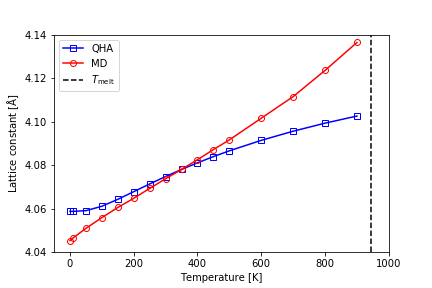
\includegraphics[width=3in]{al_therm_exp}\label{9a}}
\subfloat[]{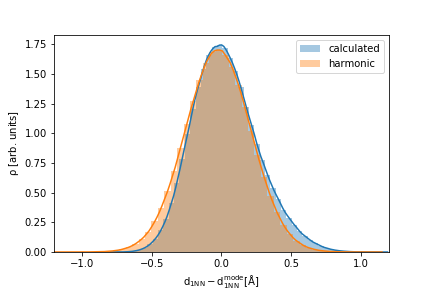
\includegraphics[width=3in]{al_bulk_anharm}\label{9b}}\hfill
\subfloat[]{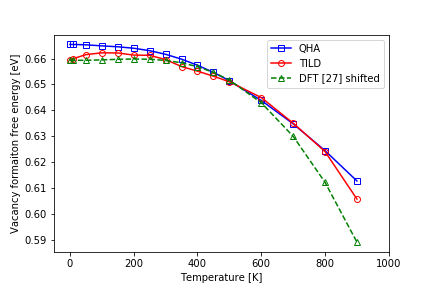
\includegraphics[width=3in]{al_vac_form}\label{9c}}
\subfloat[]{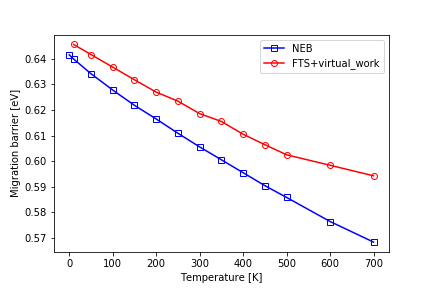
\includegraphics[width=3in]{al_vac_mig}\label{9d}}\hfill
\caption{Aluminium: (a) Thermal expansion as a function of temperature, (b) Gaussian distribution of the first NN distances around the mode of these distances at 900K, calculated using the potential \cite{Mendelev2009a} and a harmonic oscillator, (c) Vacancy formation free energy and (d) Migration barrier as a function of temperature}
\label{fig:9}
\end{figure}

\noindent Aluminium (Al) has a close-packed FCC crystal structure. The deviation of the lattice constants computed from direct MD and QHA above 400K in Fig. \ref{fig:9} (a) suggest anharmonicity in the system due to thermal expansion. This anharmonicity can be seen in Fig. \ref{fig:9} (b), where there is a shift of the first NN atoms away from their geometric position. There is a good agreement between the vacancy formation free energies from QHA and TILD in Fig. \ref{fig:9} (c), which could be a result of them being computed using different lattice constants, especially at high temperatures. The DFT curve obtained by Glesnk et al. \cite{Glensk2013} using a GGA-PBE potential in Fig. \ref{fig:9} (c) has been shifted by 0.02 eV to have the same 0K vacancy formation free energy as the TILD computed vacancy formation free energy in order to compare the obtained trends. The shifted DFT and TILD curves show a good agreement up to 600K, which shows that the classical potential does a reasonably good job in approximating the vacancy formation free energies. Using Helmholtz free energies to the Gibbs free energies also seems like a reasonable simplification at low temperatures. The deviation beyond 600K can be attributed to the outcome of this simplifying assumption, even though the deviation is small, i.e. <0.02 eV. Contrary to the Arrhenius assumption that diffusivity is a straight line in logarithmic space, and hence the vacancy migration energy is temperature independent, the temperature dependence of the vacancy migration free energies can be seen in Fig. \ref{fig:9} (d). As expected, the NEB and FTS curves deviate from each other with increasing temperature. The deviation at very low temperatures is small and could be due to the effect of smoothing the string.

The deviation from the direct MD and QHA computed lattice constants and vacancy formation energies at low temperatures, a behavior which is seen in all the simulated species, is due to the fact that direct MD does not take into account the zero point energies that are significant at these low temperatures. These are explicitly accounted for in the free energies from our QHA phonon calculations.

\begin{figure}[htp]
\centering
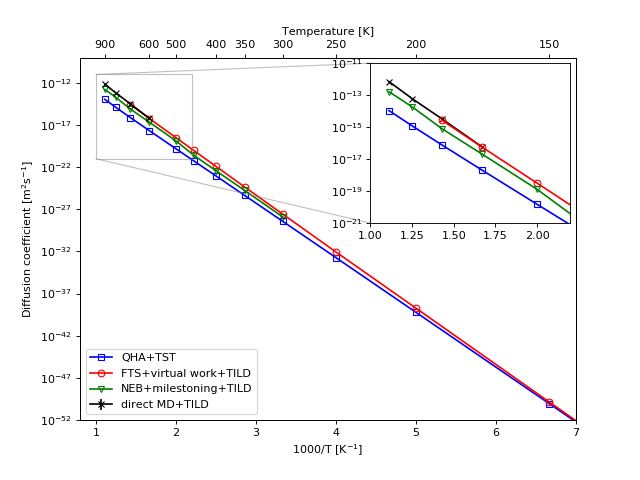
\includegraphics[scale=0.65]{al_self_diffusion}
\caption{Self-diffusion coefficient for Al computed using different methods}
\label{fig:10}
\end{figure}

The self-diffusion coefficients from direct MD for Al could only be computed down to 600K, below which no atomic migration was observed in the timescales simulated. There is a very good agreement in the self-diffusion coefficients computed using direct MD and the FTS with virtual work method at high temperatures as seen in Fig. \ref{fig:10}. There is a continuation of the FTS calculated coefficients along the slope of direct MD results all the way down to temperatures lower than room temperature. The quasi-harmonic self-diffusion coefficients deviate from the direct MD results by two orders of magnitude, while coefficients from the NEB with milestoning method are too low by about a factor of 5. This underestimation of milestoning by a factor of $\approx 5$ is a common feature among all the species.

\subsubsection{Nickel}

\begin{figure}[!htp]
\centering
\subfloat[]{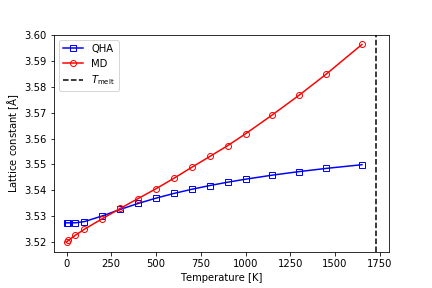
\includegraphics[width=3in]{ni_therm_exp}\label{11a}}
\subfloat[]{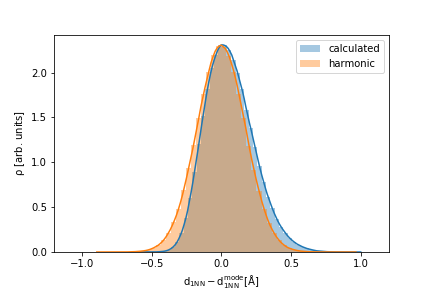
\includegraphics[width=3in]{ni_bulk_anharm}\label{11b}}\hfill
\subfloat[]{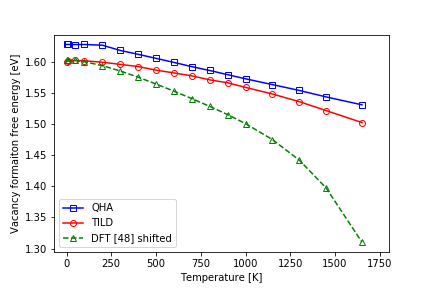
\includegraphics[width=3in]{ni_vac_form}\label{11c}}
\subfloat[]{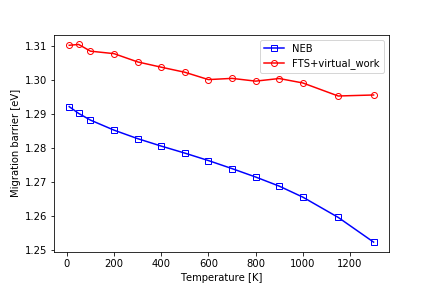
\includegraphics[width=3in]{ni_vac_mig}\label{11d}}\hfill
\caption{Nickel: (a) Thermal expansion as a function of temperature, (b) Gaussian distribution of the first NN distances around the mode of these distances at 1650K, calculated using the potential \cite{Mishin2004} and a harmonic oscillator, (c) Vacancy formation free energy and (d) Migration barrier as a function of temperature}
\label{fig:11}
\end{figure}

Similar to Al, Nickel (Ni) also has a close packed FCC crystal structure. The deviations in the lattice constants from direct MD and QHA start as low 300K, as seen in Fig. \ref{fig:11} (a). The shift of the first NN atoms away from their geometric position in Fig. \ref{fig:11} (b) shows bulk anharmonicity at high temperatures. The TILD computed vacancy formation free energies deviate from the trend of the shifted (by 0.2 eV) DFT vacancy formation free energy curve obtained by Gong et al. \cite{Gong2018} using a GGA-PBE potential, as temperature increases. Further, as can be seen in Fig. \ref{fig:11} (c), the QHA and TILD computed formation free energies decrease only by about 0.1 eV, when compared to the DFT computed formation free energies, which decrease by 0.3 eV. This deviation may be a result of using an empirical potential that does not accurately represent DFT behavior for this quantity. It may also be possible that the simplifying assumption of using Helmholtz free energies instead of Gibbs free energies is inadequate. The unevenness in the migration barrier computed from FTS compared to the barrier obtained from NEB in Fig. \ref{fig:11} (d) can be attributed to thermal noise, as the magnitude by which the barrier varies with temperature is about 0.01 eV. However, the trend of the FTS curve still deviates from the NEB curve as expected, similar to Al. In this case, FTS also overestimates the migration barrier at very low temperatures by about 0.03 eV. As indicated in the case of Al, deviations from the NEB migration barriers at very low temperatures can be caused by smoothing the string. However, as can be seen in section \ref{smooth}, a deviation of 0.03 eV is large for a nominal smoothing of 0.1. A possible reason could be that the number of string updates towards the running average of the images is insufficient.

\begin{figure}[htp]
\centering
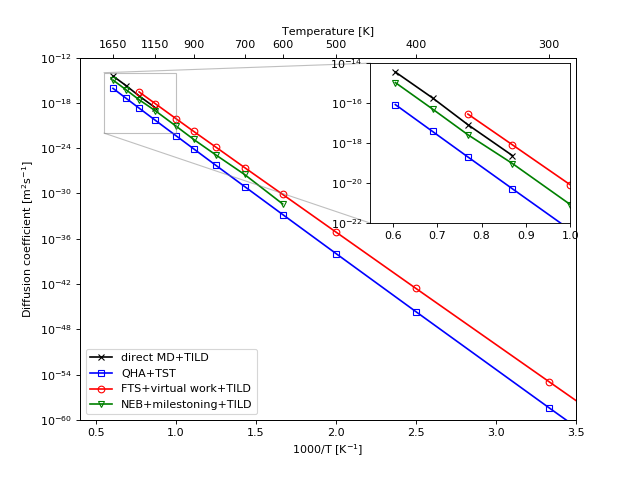
\includegraphics[scale=0.65]{ni_self_diffusion}
\caption{Self-diffusion coefficient for Ni computed using different methods}
\label{fig:12}
\end{figure}

Atomic migration for Ni was obtained only above 1150K, which is why self-diffusion coefficients from direct MD could only be obtained beyond this temperature. This shows the limitations of the direct MD method for computing quantities like diffusion coefficients. The self-diffusion coefficients from the FTS with virtual work method are larger by a factor of 5 from the direct MD coefficients at 1250K, and this trend continues down to lower temperatures, as seen in Fig. \ref{fig:12}. The slight overestimation of the self-diffusion coefficient computed using the FTS with virtual work method when compared to direct MD at high temperatures, could be associated to the assumption in Eyring's reaction rate theory, that once the migration barrier is crossed, diffusion always takes place. The quasi-harmonic self-diffusion coefficients deviate from the direct MD results by about two orders of magnitude at high temperatures and further at lower temperatures, while the NEB with milestoning results are lower by about a factor of 5 from the direct MD results.

\subsubsection{Copper}

\begin{figure}[!htp]
\centering
\subfloat[]{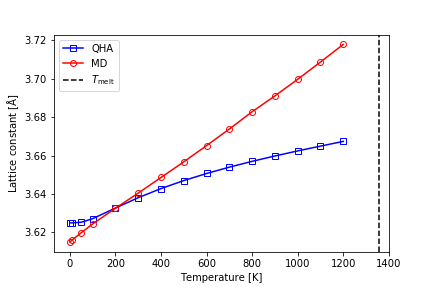
\includegraphics[width=3in]{cu_therm_exp}\label{13a}}
\subfloat[]{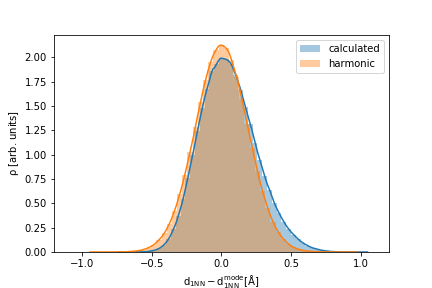
\includegraphics[width=3in]{cu_bulk_anharm}\label{13b}}\hfill
\subfloat[]{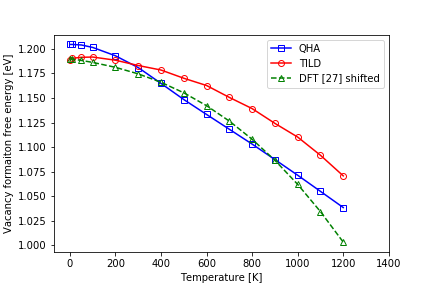
\includegraphics[width=3in]{cu_vac_form}\label{13c}}
\subfloat[]{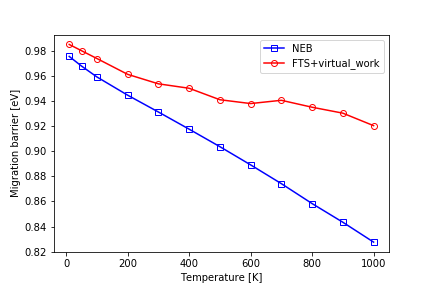
\includegraphics[width=3in]{cu_vac_mig}\label{13d}}\hfill
\caption{Copper: (a) Thermal expansion as a function of temperature, (b) Gaussian distribution of the first NN distances around the mode of these distances at 1200K, calculated using the potential \cite{Mendelev2008} and a harmonic oscillator, (c) Vacancy formation free energy and (d) Migration barrier as a function of temperature}
\label{fig:13}
\end{figure}

Copper (Cu) which also has a close packed FCC crystal structure, shows a thermal expansion behavior similar to Ni: the lattice constants from direct MD and QHA shown in Fig. \ref{fig:13} (a) start deviating at around 200K, giving a maximum deviation of about 0.05 eV at the highest simulated temperature of 1200K. Cu also exhibits similar anharmonic behavior as Al and Ni, wherein the first NN atoms move away from their geometric position as seen in Fig. \ref{fig:13} (b). The vacancy formation free energies computed from TILD in Fig. \ref{fig:10} (c) follow a different trend from the QHA ones. The deviation between the TILD computed vacancy formation free energies and the trend of the shifted (by 0.1 eV) DFT formation free energies obtained by Glesnk et al. \cite{Glensk2013} from a GGA-PBE potential increases with increasing temperature, similar to that observed for Ni. However, the change in the formation free energies from the two curves with increasing temperature is comparable. This may once again be a result of using a DFT inaccurate potential. There is a significant deviation in the migration barrier from NEB to the the one computed using FTS, with increasing temperature showing clearly that the transition paths computed by the two methods are significantly different. FTS once again overestimates the migration barrier at very low temperatures by about 0.02 eV. 

\begin{figure}[htp]
\centering
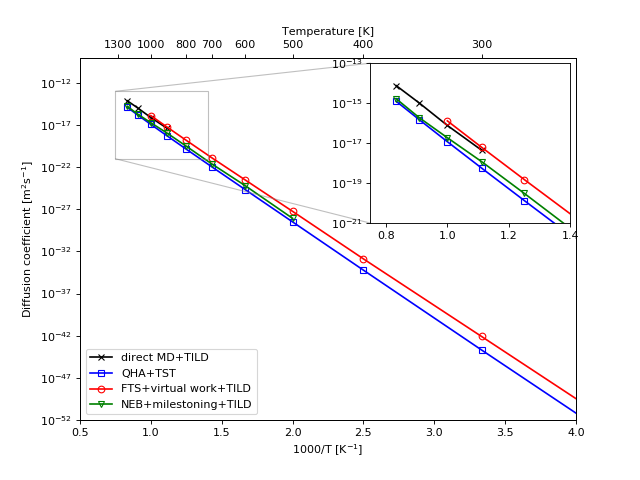
\includegraphics[scale=0.65]{cu_self_diffusion}
\caption{Self-diffusion coefficient for Cu computed using different methods}
\label{fig:14}
\end{figure}

No atomic migration could be simulated below 900K using direct MD. Like Al, an excellent agreement between the direct MD and FTS computed self-diffusion coefficients can be observed at high temperatures in Fig. \ref{fig:14} with a very slight overestimate. The FTS computed coefficients continue along the slope of the direct MD coefficients to lower temperatures. The quasi-harmonic self-diffusion coefficients deviate from the direct MD results by less than an order of magnitude at high temperatures and deviate further at lower temperatures, and the NEB with milestoning method is lower yet again by about a factor of 5 from the direct MD results, which suggests that some quantity is not being accounted for.

\subsubsection{Iron}

\begin{figure}[!htp]
\centering
\subfloat[]{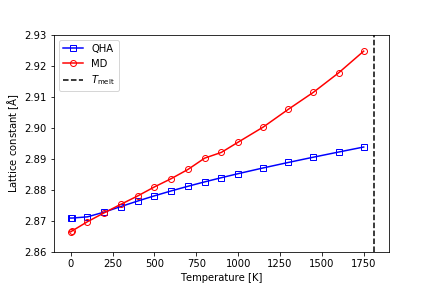
\includegraphics[width=3in]{fe_therm_exp}\label{13a}}
\subfloat[]{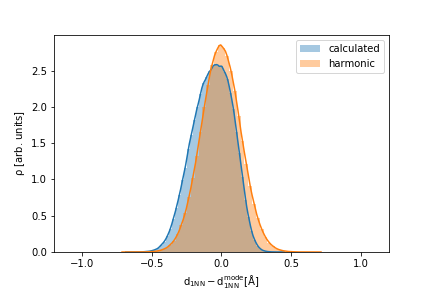
\includegraphics[width=3in]{fe_bulk_anharm}\label{13b}}\hfill
\subfloat[]{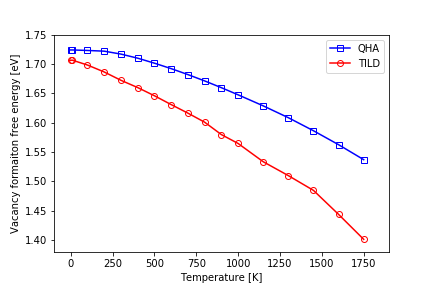
\includegraphics[width=3in]{fe_vac_form}\label{13c}}
\subfloat[]{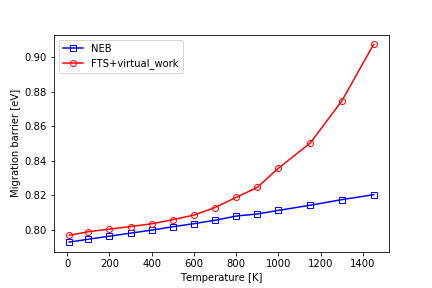
\includegraphics[width=3in]{fe_vac_mig}\label{13d}}\hfill
\caption{Iron: (a) Thermal expansion as a function of temperature, (b) Gaussian distribution of the first NN distances around the mode of these distances at 1750K, calculated using the potential \cite{Ackland1997} and a harmonic oscillator, (c) Vacancy formation free energy and (d) Migration barrier as a function of temperature}
\label{fig:15}
\end{figure}

Iron (Fe) has a less dense BCC crystal structure as its stable structure. Deviation between the lattice constants computed from direct MD and QHA start at 200 K as shown in Fig. \ref{fig:15} (a). Unlike the species with an FCC structure, the first NN distance seems to decrease from the geometric first NN distance with increasing temperature, which means the first NN atoms move towards the atom as temperature increases. The shift of the peak of the Gaussian distribution in Fig. \ref{fig:15} (b) and the corresponding negative skewness of the distribution is further evidence of this attractive behavior between the Fe atoms. A possible explanation for this could be the large cohesive energy of the Fe atoms (-4.3 eV / atom \cite{Ackland1997}). Cohesive energies of the species may be helpful in understanding bulk anharmonic behavior, and is discussed in more detail in section \ref{bulk_anharm}. As shown in Fig. \ref{fig:15} (c), the TILD vacancy formation free energies deviate even at low temperatures form the QHA computed formation free energies, and drop significantly with increasing temperature, by about 0.3 eV from the 0K formation energies. The increase in the trend of the migration barriers  in Fig. \ref{fig:15} (d) with increasing temperature can be justified by using the observation that first NN atoms move towards a given atom: as temperature increases, the atoms are much closer to each other and tightly bound, thus creating a less favorable local energy landscape along which the NN atom has to traverse to migrate to a vacancy site. After a constant deviation of 0.012 eV up to 600K, the FTS and NEB computed migration barriers deviate significantly.

\begin{figure}[htp]
\centering
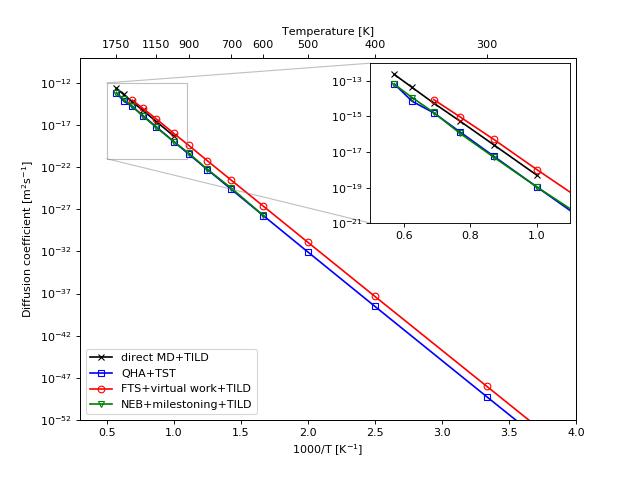
\includegraphics[scale=0.65]{fe_self_diffusion}
\caption{Self-diffusion coefficient for Fe computed using different methods}
\label{fig:16}
\end{figure}

The self-diffusion coefficients computed using different methods are shown in Fig. \ref{fig:16}. Right away, it its noticeable that the difference between the direct MD and QHA computed coefficients is smaller than the difference for the FCC species. This can be understood as a cancellation of errors: since the vacancy formation free energy decreases and vacancy migration free energy remains almost constant with increasing temperature, the errors from the quasi-harmonic method would cancel out to give a diffusion coefficient that agrees well with direct MD. The self-diffusion coefficient computed from the NEB with milestoning method is sill lower by about a factor of 5 at high temperatures, which in this case also happens to be the same factor by which the quasi-harmonic coefficients are lower by.

\subsubsection{Molybdenum}

\begin{figure}[!htp]
\centering
\subfloat[]{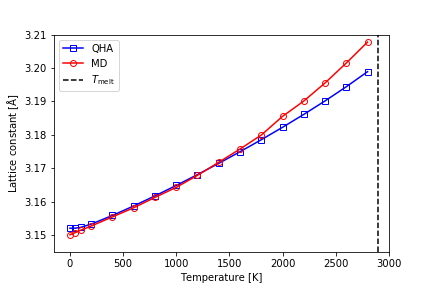
\includegraphics[width=3in]{mo_therm_exp}\label{13a}}
\subfloat[]{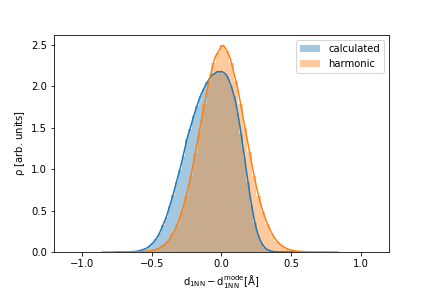
\includegraphics[width=3in]{mo_bulk_anharm}\label{13b}}\hfill
\subfloat[]{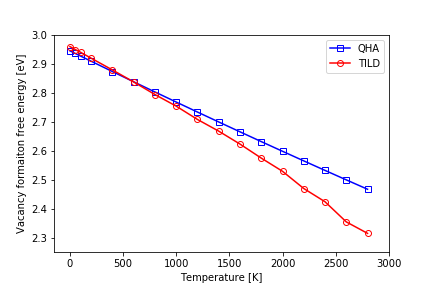
\includegraphics[width=3in]{mo_vac_form}\label{13c}}
\subfloat[]{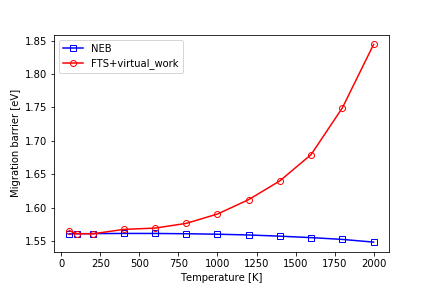
\includegraphics[width=3in]{mo_vac_mig}\label{13d}}\hfill
\caption{Molybdenum: (a) Thermal expansion as a function of temperature, (b) Gaussian distribution of the first NN distances around the mode of these distances at 2800K, calculated using the potential \cite{Zhou2004} and a harmonic oscillator, (c) Vacancy formation free energy and (d) Migration barrier as a function of temperature}
\label{fig:17}
\end{figure}

Molybdenum (Mo), which has a high melting temperature of 2896K has a stable BCC crystal structure. When compared to the other species studied in this thesis so far, the lattice constants obtained from direct MD and QHA for Mo are in every good agreement up to 1600K, beyond which they deviate slightly giving a maximum deviation of 0.01eV at the 2800K, as seen in Fig. \ref{fig:17} (a). The behavior where the first NN atoms move towards the atom as temperature increases as seen in Fe, is also seen in Mo, as can be inferred from the Fig. \ref{fig:17} (b). The vacancy formation energies from TILD have the same trend as Fe but agree with QHA computed formation free energies below 500K as shown in Fig. \ref{fig:17} (c). From Fig. \ref{fig:17} (d), the migration barrier for Mo grows quickly by about 0.3 eV from 0 to 0.75 $T_{\mathrm{melt}}$ when compared to Fe, where it increases by 0.05 eV for the same range. The NEB computed migration barrier meanwhile, remains almost a constant.

\begin{figure}[htp]
\centering
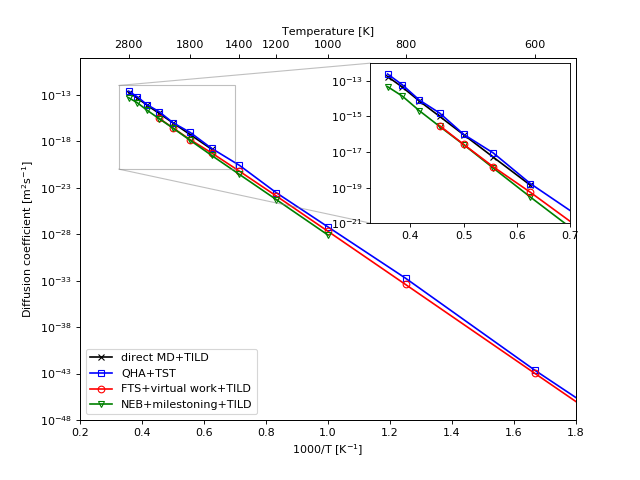
\includegraphics[scale=0.65]{mo_self_diffusion}
\caption{Self-diffusion coefficient for Mo computed using different methods}
\label{fig:18}
\end{figure}

As can be seen in Fig. \ref{fig:18}, the self-diffusion coefficients for Mo from direct MD show a very good agreement with the coefficients from the quasi-harmonic method. This is not surprising, since thermal expansion data from the two methods only deviate at very high temperatures. In addition to this more harmonic behavior, it is also possible at the highest temperatures that such good agreement between the direct MD and quasi-harmonic data is because of the cancellation of errors of the vacancy formation and migration free energies. The underestimation of the coefficients at high temperatures from the FTS with virtual work method is a direct outcome of the rapidly increasing migration barriers with increasing temperature. While it is expected that the transition pathway remain symmetric at convergence and increase in a predictable manner as can be seen at low temperatures for Mo in Fig. \ref{fig:19}, the pathway for Mo with increasing temperatures shows an asymmetry pointing out clear convergence issues. The NEB with milestoning self-diffusion coefficients are consistently lower by a factor of 5 at high temperatures.

\begin{figure}[!htp]
\centering
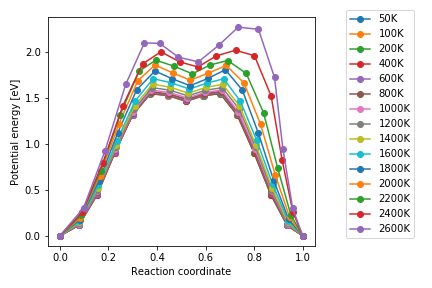
\includegraphics[scale=0.65]{migration_barriers}
\caption{Transition pathways for Mo at different temperatures using the FTS method. Non-convergence of the string is evident at high temperatures}
\label{fig:19}
\end{figure}

\subsection{Observed trends}

\subsubsection{Bulk anharmonicity}\label{bulk_anharm}

\begin{figure}[htp]
\centering
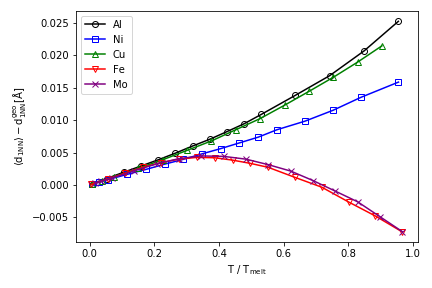
\includegraphics[scale=0.65]{bulk_anharm_all}
\caption{Bulk anharmonicity, expressed as the difference in $\mathrm{\AA}$ between the expected first NN distance ($\langle \mathrm{d_{1NN}} \rangle$) and the geometric first NN distance calculated from the temperature dependent lattice constants ($\mathrm{d_{1NN}^{geo}}$) against fraction of melting temperature}
\label{fig:20}
\end{figure}

From the Gaussian distributions of the first NN distances of different species (Figs. (b) of the respective species), two different trends can be observed at the highest simulated temperatures of the species: the first NN atoms move away from the atom, as seen in from the distributions of Al, Ni and Cu (FCC species) and the first NN atoms move towards the atom, as seen in the distributions of Fe and Mo (BCC species). Fig. \ref{fig:20} shows the relative shift of the first NN atoms from their geometric position (obtained from the temperature dependent lattice constants) against the fraction of melting temperature. This shift is considered as a measure of the bulk anharmonicity of a species. It can be seen that for the FCC species, the relative shift is 0 at the lowest temperature and increases with increasing temperature. Al shows the highest shift since it has the weakest cohesive energy ($-3.411$ eV / atom \cite{Mendelev2009a}), followed by Cu ($-3.49$ eV / atom \cite{Mendelev2008}) and Ni ($-4.45$ eV / atom \cite{Mishin2004}). For the BCC species on the other hand, the first NN atoms seem to move slightly away from the atom and then move closer towards the atom at elevated temperatures as observed from the distributions. This can also be attributed to the string cohesive energies of the BCC species, Fe ($-4.316$ eV / atom  \cite{Ackland1997}) and Mo ($-6.82$ eV / atom \cite{Zhou2004}). Because the cohesive energy for Ni is stronger than that of Fe, this energy alone is not a complete explanation, but the relative geometries of the two crystal structure must also play a role.

\subsubsection{Vacancy anharmonicity and vacancy formation energies}

\begin{figure}[!htp]
\centering
\subfloat[]{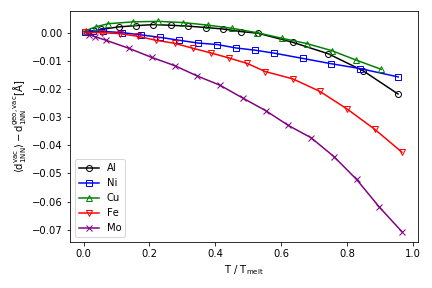
\includegraphics[width=3in]{vac_anharm_all}\label{20a}}
\subfloat[]{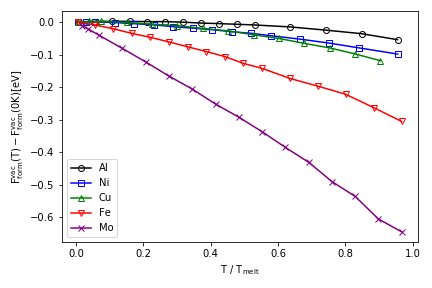
\includegraphics[width=3in]{vac_form_all}\label{20b}}\hfill
\caption{(a) Anharmonicity due to vacancy, expressed as the difference in $\mathrm{\AA}$ between the expected first NN distance ($\langle \mathrm{d_{1NN}^{vac}} \rangle$) to the vacancy and the geometric first NN distance to the vacancy calculated from the temperature dependent lattice constants ($\mathrm{d_{1NN}^{geo, vac}}$) against fraction of melting temperature, (b) The relative change in vacancy formation free energies as a function of temperature against fraction of melting temperature}
\label{fig:21}
\end{figure}

When a vacancy is created in a structure, the NN atoms relax towards that vacancy. The anharmonic contribution to this relaxation is shown in Fig. \ref{fig:21} (a), by taking the relative shift of the first NN atoms to the vacancy from their geometric position to the vacancy as a function of fraction of melting temperature.. The resulting curves have almost the same trends as the relative change in vacancy formation free energies, calculated as the difference between the temperature dependent vacancy formation free energies and the vacancy formation free energy at 0 K lattice, shown in Fig. \ref{fig:21} (b). This can be interpreted as follows: the FCC atoms have comparatively weak relaxations away from, then towards the vacancy. The formation energy (compared to the reference) is only weakly dependent on temperature, and only at very large fractions of $T_{\mathrm{melt}}$ does it really starts to drop. On the other hand, BCC atoms relax towards the vacancy quite strongly -- i.e. they \enquote*{like} it -- and indeed, the formation energy drops to match.


\subsubsection{Effect of sampling period}\label{sample}

\begin{figure}[!htp]
\centering
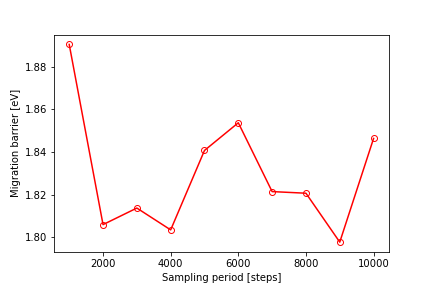
\includegraphics[scale=0.65]{sample_bcc}
\caption{Effect of sampling period on the migration energy of Mo at 2000K}
\label{fig:22}
\end{figure}

As stated in section \ref{cas}  - Vacancy migration free energy, the highest simulated temperature was restricted to 0.75 $T_{\mathrm{melt}}$. At temperatures close to the melting point, the atoms within the crystal structure vibrate with large amplitudes, thus resulting in a fluctuating total energy of the structure. Within the FTS method, this fluctuation translates as the centroids having a lot more freedom to explore its Voronoi cell, which includes high energy potential regions. If the running average of the centroid is mixed too often with the centroid during string evolution, the centroid can get \enquote*{stuck} in such a high energy region. Because of its high energy at high temperatures, the centroid will continue evolving in the same manner with every update, thereby never converging to the minimum free energy path. The effect of the sampling period on the migration barrier is shown in Fig. \ref{fig:22}. Even at high sampling periods of up to 10000 steps, convergence is not achieved. As the string needs to be updated toward the running average of the images at least 100 times for a good convergence to the minimum free energy path increasing this sampling period beyond 10000 steps becomes computationally impractical. At lower temperatures however, a lower sampling period (5000 steps in this thesis) is sufficient to obtain a good convergence of the string. 

\clearpage
\section{Conclusion}

The finite temperature string (FTS) method has been used to along with the virtual work principle and thermodynamic integration (TILD) to obtain fully anharmonic self-diffusion coefficients from 1K up to 0.75 $\mathrm{T_{melt}}$ for Al, Ni, Cu, Fe and Mo. In addition, self-diffusion coefficients from direct molecular dynamics (direct MD) simulations, the quasi-harmonic method and the nudged elastic band with milestoning method are also obtained. A near perfect agreement is obtained for Al, Cu and Fe between the FTS and direct MD at high temperatures, while Ni is only slightly overestimated and Mo shows non-Arrhenius behavior at high temperatures. The coefficeints from the FTS method show a significant improvement from the coefficients computed using the quasi harmonic method at high temperatures. The coefficients from the NEB with milestoning method are lower than the direct MD coefficients by about a factor of 5 for all species. This consistency across so many species implies that there is some key component missing, either in the method or in its implementation.

Non-convergence of the FTS string at temperatures greater than 0.75 $\mathrm{T_{melt}}$ can be associated to the inadequate sampling within the Voronoi cell during string evolution. The migration barriers computed from the FTS method deviate from those obtained from the NEB method with increasing temperature for all the species, as expected.

The bulk anharmonic contribution during thermal expansion seems to depend on the cohesive energies between the atoms in the structure, wherein atoms with the least negative cohesive energies show greater anharmonicity. The anharmonic contribution due to the vacancy is much higher in the BCC species than in the FCC species. The vacancy formation free energies computed from TILD change by only a small fraction with increasing temperature for the FCC species, while those computed for the BCC species change significantly. \\


\clearpage
\section{Future outlook}

The finite temperature string method can be used to predict self-diffusion coefficients for FCC and BCC species up to 0.75 $\mathrm{T_{melt}}$. Beyond this temperature however, the FTS fails to converge to the transition path within a reasonable sampling period and number of string updates. A good first step to determining the cause for this non-convergence would be to run at higher sampling periods ($>$ 10000 steps) for a high temperature to see if low sampling period is indeed the underlying cause for this non-convergence. Since there is near perfect agreement between direct MD and FTS computed self-diffusion coefficients for species like Al, Cu and Fe, if the reason behind the offset for Ni and the convergence issues for Mo can be found and rectified, the FTS method can be applied to any metallic system with a semi-empirical classical potential. The computation of self-diffusion coefficients using direct MD with TILD, the quasi harmonic method, the FTS with virtual work method and TILD, and the NEB with milestoning method and TILD, have been implemented in an easy collection of notebooks that can be run using pyiron. 

The seemingly constant shift of the NEB with milestoning result from direct MD is very suspicious and necessitates further investigation. To test the robustness of the FTS method across all species, the inclusion of non-FCC and BCC species is also necessary, e.g. for HCP species which have the complicating factor of in- and out-of-plane migration jumps.

Given that the TILD and FTS methods used in this thesis only calculates Helmholtz free energies of vacancy formation and migration respectively, a look into computing the Gibbs free energies is also an important next step. The deviations seen in Ni and Mo self-diffusion coefficients could be rectified by using the Gibbs free energies of vacancy migration over the Helmholtz free energies.

The results obtained in this thesis are not compared against experimental results, primarily because the results obtained are as good as the potential used to simulate them. In order to draw a comparison with experimental results, it is necessary to use DFT, or DFT-accurate potentials. However, because of run times almost as expensive as direct MD, using FTS with such potentials is still computationally impractical. An alternative to DFT accurate potentials are machine learned potentials (MLPs), can be trained on-the-fly to reproduce DFT forces and energies, e.g. \cite{Gubaev2018}. This will also be a prime focus of future work with this method.

\clearpage
\section{Acknowledgements}

I would sincerely like to extend my heartfelt gratitude to Prof. Dr. Jörg Neugebauer (MPIE) and Prof. Dr. Robert Spatscheck (FZ Jülich, RWTH Aachen) for this opportunity to write my Master's thesis with them. Very few persons are able to grasp complex scientific ideas in such short time and suggest a way forward as them. I thank Prof. Dr. Blazej Grabowski (MPIE, Stuttgart University) for having that initial faith in me that I could work on this topic, and for those short yet very illuminating discussions paving the way forward for this work. I thank PD Dr. Denis Music (Materials Chemistry, RWTH Aachen) for all his help and suggestions with the administrative part of writing an external Master's thesis.

Dr. Liam Huber (MPIE) deserves a paragraph of his own; there are very few bosses who are as patient, understanding and intelligent as Dr. Huber. I thank him for instilling in me the desire to understand why things work the way they do, and not simply take for granted that they work. Credit goes to him for making me think more like a physicist and less like an engineer (in applicable circumstances). From discussions on coding etiquette, server crashing, shaking heads because I understand less physics than he does, letting me use some of his well-written-yet-to-be-published text for presentations, to fruitful discussions on understanding each of the elements of all the work that makes up this thesis, Dr. Huber has been more of a friend than a boss to me. For this, I will be always grateful to him.

I thank my colleagues at MPIE, especially Jan Janßen, for his constant efforts in making pyiron as easy to use as possible, Dr. Osamu Waseda and Dr. Eunan McEniry, for their interesting insight into the applications of the FTS method, transition pathways and constrained MD. To Dominik Gehringer, who along with Dr. Huber and Jan Janßen implemented \enquote*{protocols} in pyiron. A shout out to my boy Ananya Kumar Singh, who was always very patient with me when I needed a refresher on basic topics in mathematics and solid state physics, and on life in general. 

As this thesis marks the end of my time as a Master's student at the RWTH, I would like to briefly mention a few people who have played a behind-the-scenes role in helping me be where I am today: my parents, for trusting me enough to not ask too many questions on what I have been up to in Germany for the last three years, my sister, for being a secondary bank account, Nitesh, Karthik, Harsh, Daniel, Sharmistha, Romana and Sebastian for still being friends with me, even after my constant refusals to meet up because I had to work on this thesis, Julita, for rekindling my love for music to find peace during my blue days with FTS, and Anush,a for being an amazing person.

\clearpage
\section{Declaration of originality}

I, Raynol Dsouza, hereby confirm that unless stated otherwise, this work is the result of my own efforts. These efforts include the originality of written sections, figures or similar pictorial material and results. Where material is drawn from other sources, references have been included. \\
\\
\\
\flushright(Raynol Dsouza)


\newpage
\bibliography{citations} 
\bibliographystyle{ieeetr}

\newpage
\section{Appendix}

\subsection{Effect of number of images}

\begin{figure}[!htp]
\centering
\subfloat[]{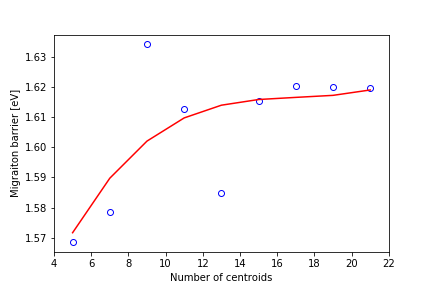
\includegraphics[width=3in]{n_images_bcc}\label{22a}}
\subfloat[]{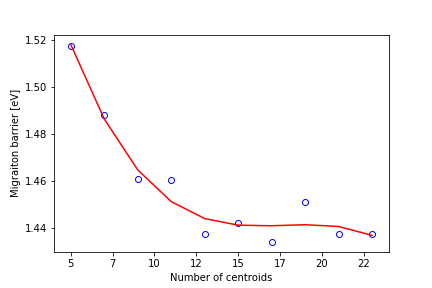
\includegraphics[width=3in]{n_images_fcc}\label{22b}}\hfill
\caption{Effect of the number of images on the migration energies for (a) FCC (Ni at 1K) and (b) BCC (Mo at 1K) crystal structures}
\label{fig:23}
\end{figure}

Since the transition path obtained from the FTS method is not fitted to obtain the migration barrier, it is important to use a sufficient number of centroids which make up the string. As can be seen in Fig. \ref{fig:23}, too few centroids give the wrong migration energies, because the path along which virtual work is computed is too sparse. On the other hand, using too many centroids increases computational costs. In this work, 13 centroids for FCC structures and 15 images for BCC structures are used.

\subsection{Effect of smoothing}\label{smooth}

\begin{figure}[!htp]
\centering
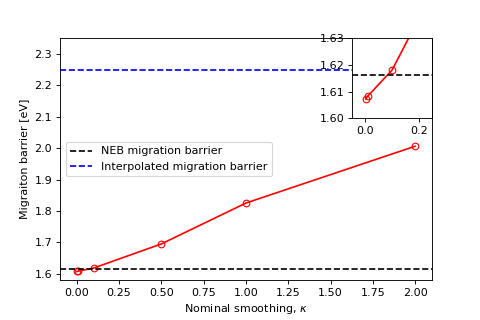
\includegraphics[scale=0.65]{smooth}
\caption{Effect of nominal smoothing on the migration energy of Mi at 1K}
\label{fig:24}
\end{figure}

The amount of smoothing applied to the string during its evolution also plays a role in determining the correct migration barrier. Fig. \ref{fig:24} shows the increase in the migration barrier with increasing nominal smoothing of 0.001, 0.01, 0.1 and 1. At maximum nominal smoothing, the string should be the same as the interpolated string between the equilibrium vacancy structures. Since the potential energy landscape for vacancy diffusion is not as rough as the landscapes for which FTS was originally designed to be applied, a very low nominal smoothing of 0.01 is used in this work.

\subsection{TILD Integrands}

The integrands obtained from the TILD method for the decoupling between the vacancy with one harmonic oscillator structure and the EAM structure are shown in the Fig. \ref{fig:25}. A left bias is applied such that the lambdas are more concentrated towards the vacancy with the harmonic oscillator structure. Using 8 and 16 discreet coupling strengths does not affect the integrands by much, except at the lambda = 0 region, where the extra points from the 16 resolve better.

\begin{figure}[!htp]
\centering
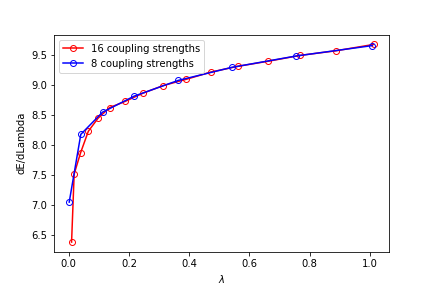
\includegraphics[scale=0.65]{lambdas}
\caption{Integrand vs. Lambdas from TILD at 2000K for Mo}
\label{fig:25}
\end{figure}

\subsection{Code examples}

Each of the nodes used in the FTS and Markovian milestoning algorithms were defined as classes within pyiron. The code for three of these classes, StringReflect, CentroidsSmoothing and Reparameterize, is shown below:

\subsubsection{Reflect - String}

\begin{lstlisting}
class StringReflect(StringDistances):

    """
    If not, the image's positions, velocities and forces are reset to the previous time step.
    Input attributes:
        positions (numpy.ndarray): Atomic positions of the image.
        velocities (numpy.ndarray): Atomic velocities of the image.
        forces (numpy.ndarray): Atomic forces of the image.
        previous_positions (numpy.ndarray): Atomic positions of the image from the previous time step.
        previous_velocities (numpy.ndarray): Atomic velocities of the image from the previous time step.
        previous_velocities (numpy.ndarray): Atomic velocities of the image from the previous time step.
        centroid_positions (numpy.ndarray): The positions of the image's centroid.
        all_centroid_positions (list/numpy.ndarray): A list of positions for all centroids in the string.
        cell (numpy.ndarray): The 3x3 cell vectors for periodic boundary conditions.
        pbc (numpy.ndarray): Three booleans declaring which dimensions have periodic boundary conditions for finding
            the minimum distance convention.
        eps (float): The maximum distance between the closest centroid and the parent centroid to be considered a match
            (i.e. no reflection of image necessary). (Default is 1e-6.)

    Output attributes:
        positions (numpy.ndarray): Either the original positions passed in, or the previous ones.
        velocities (numpy.ndarray): Either the original velocities passed in, or the previous ones.
        forces (numpy.ndarray): Either the original forces passed in, or the previous ones.
        reflected (bool): Whether or not the image got reflected.
    """
    
    def __init__(self, name=None):
        super(StringReflect, self).__init__(name=name)

    def command(self, positions, velocities, forces, previous_positions, previous_velocities, previous_forces,
                centroid_positions, all_centroid_positions, cell, pbc, eps):
        
        # Check if the image is closest to its parent centroid or not. Returns a boolean.
        if self.check_closest_to_parent(positions, centroid_positions, all_centroid_positions, cell, pbc, eps):
            return {
                'positions': positions,
                'velocities': velocities,
                'forces': forces,
                'reflected': False
            }
        else:
            return {
                'positions': previous_positions,
                'velocities': -previous_velocities,
                'forces': previous_forces,
                'reflected': True
            }
\end{lstlisting}

\subsubsection{Smooth}

\begin{lstlisting}
class CentroidsSmoothing(PrimitiveVertex):

    """
    Global smoothing following Vanden-Eijnden and Venturoli (2009). The actual smoothing strength is the product of the
    nominal smoothing (`kappa`), the number of images, and the mixing fraction (`dtau`).
    Input Attributes:
        kappa (float): Nominal smoothing.
        dtau (float): Mixing fraction (from updating the string towards the running average of the image positions).
        all_centroid_positions (list/numpy.ndarray): List of all the centroid positions along the string.

    Output Attributes:
        all_centroid_positions (list/numpy.ndarray): List of smoothed centroid positions.
    """

    def command(self, kappa, dtau, all_centroid_positions):

        n_images = len(all_centroid_positions)
        smoothing_strength = kappa * n_images * dtau
        smoothing_matrix = self._get_smoothing_matrix(n_images, smoothing_strength)
        smoothed_centroid_positions = np.tensordot(smoothing_matrix, np.array(all_centroid_positions), axes=1)

        return {
            'all_centroid_positions': smoothed_centroid_positions
        }

    @staticmethod
    def _get_smoothing_matrix(n_images, smoothing_strength):

        """
        A method that returns the smoothing matrix used in centroid smoothing.

        Attributes:
            n_images (int): number of images
            smoothing_strength (float): the smoothing penalty

        Returns:
            [n_images x n_images] smoothing_matrix
        """

        toeplitz_rowcol = np.zeros(n_images)
        toeplitz_rowcol[0] = -2
        toeplitz_rowcol[1] = 1
        second_order_deriv = toeplitz(toeplitz_rowcol, toeplitz_rowcol)
        second_order_deriv[0] = np.zeros(n_images)
        second_order_deriv[-1] = np.zeros(n_images)
        smooth_mat_inv = np.eye(n_images) - smoothing_strength * second_order_deriv

        return np.linalg.inv(smooth_mat_inv)
\end{lstlisting} 

\subsubsection{Reparameterize}

\begin{lstlisting}
class CentroidsReparameterization(PrimitiveVertex):
    """
    Use linear interpolation to equally space the centroids between the first and last centroid in 3N dimensional space,
    using a piecewise function

    Input attributes:
        all_centroid_positions (list/numpy.ndarray): List of all the centroids along the string
        cell (numpy.ndarray): The cell of the structure
        pbc (numpy.ndarray): Periodic boundary condition of the structure

    Output attributes:
        all_centroid_positions (list/numpy.ndarray): List of equally spaced centroids
    """

    def __init__(self, name=None):
        super(CentroidsReparameterization, self).__init__(name=name)

    def command(self, all_centroid_positions, cell, pbc):

        # How long is the piecewise parameterized path to begin with?
        lengths = self._find_lengths(all_centroid_positions, cell, pbc)
        length_tot = lengths[-1]
        length_per_frame = length_tot / (len(all_centroid_positions) - 1)

        # Find new positions for the re-parameterized centroids
        new_positions = [all_centroid_positions[0]]
        for n_left, cent in enumerate(all_centroid_positions[1:-1]):
            n = n_left + 1
            length_target = n * length_per_frame

            # Find the last index not in excess of the target length
            try:
                all_not_over = np.argwhere(lengths < length_target)
                highest_not_over = np.amax(all_not_over)
            except ValueError:
                # If all_not_over is empty
                highest_not_over = 0

            # Interpolate from the last position not in excess
            start = all_centroid_positions[highest_not_over]
            end = all_centroid_positions[highest_not_over + 1]
            disp = find_mic(end - start, cell, pbc)[0]  # from ase.geometry
            interp_dir = disp / np.linalg.norm(disp)
            interp_mag = length_target - lengths[highest_not_over]

            new_positions.append(start + interp_mag * interp_dir)
        new_positions.append(all_centroid_positions[-1])

        # Apply the new positions all at once
        all_centroid_positions = new_positions

        return {
            'all_centroid_positions': all_centroid_positions
        }

    @staticmethod
    def _find_lengths(a_list, cell, pbc):
        """
        Finds the cummulative distance from job to job.

        Attribute:
            a_list (list/numpy.ndarray): List of positions whose lengths are to be calculated
            cell (numpy.ndarray): The cell of the structure
            pbc (numpy.ndarray): Periodic boundary condition of the structure

        Returns:
            lengths (list): Lengths of the positions in the list
        """
        length_cummulative = 0
        lengths = [length_cummulative]
        # First length is zero, all other lengths are wrt the first position in the list
        for n_left, term in enumerate(a_list[1:]):
            disp = find_mic(term - a_list[n_left], cell, pbc)[0]
            length_cummulative += np.linalg.norm(disp)
            lengths.append(length_cummulative)
        return lengths
\end{lstlisting}

\end{document}